\documentclass[11pt,a4paper,titlepage]{report}

\usepackage{url}
\usepackage{csquotes}
\usepackage[backend=biber, style=trad-abbrv]{biblatex}
\usepackage{amsmath}
\usepackage{amssymb}
\usepackage{graphicx}
\usepackage{siunitx}
\usepackage{listings}
\usepackage{titling}
\usepackage{pdfpages}
\newcommand{\subtitle}[1]{%
	\posttitle{%
		\par\end{center}
	\begin{center}\large#1\end{center}
	\vskip0.5em}%
}
\lstset{
	frame=tb,
	language=c,
	aboveskip=3mm,
	belowskip=3mm,
	showstringspaces=false,
	columns=flexible,
	basicstyle={\small\ttfamily},
	numbers=left,
	breaklines=true,
	breakatwhitespace=true,
	tabsize=3
}

\title{Final Project}
\subtitle{Autonomous Underwater Vehicle}
\author{Richard Sefton}

\graphicspath{./assets/}
\usepackage[inkscapeformat=png]{svg}

\addbibresource{BIBLIOGRAPHY.bib}

\setcounter{chapter}{1}

\begin{document}
	\maketitle
	\tableofcontents
	
	\begin{abstract}
		This report depicts the end to end design and development of an Autonomous Underwater Vehicle for the Final Project of the BSc Computer Science degree. As it transpires this was an incredibly ambitious project to deliver in such a short time frame. This report will try to capture the key aspects of the development process which will be a challenge in itself given the constraints on the report and as such, some aspects will be focused on more than others.  
	\end{abstract}
	
	\chapter*{Introduction} (max 2 pages)
	\addcontentsline{toc}{chapter}{Introduction}
	Autonomous Underwater Vehicles have been around since the 1950s, with the first AUV on record developed by Washington University in 1957 named SPURV\cite{SPURV} (Self Propelled Underwater Research Vehicle). The device was fitted with various temperature and pressure sending probes and could traverse to depths of 3600\unit{\meter} and one of the last uses of the SPURV AUV was to study submarine wakes in the 70s. Since this first development, in the last 67 years AUVs have been refined and further developed by various governments, oceanographic institutes, universities and private companies. Today, AUVs are often considered cheaper, better and safer to deploy than manned underwater vehicles (particularly in the light of the more recent Titan submarine implosion\cite{TITAN_IMPLOSION}), and safer than deploying divers. They are capable of obtaining more data than any single diver can obtain, and capable of diving longer than any manned vehicle as the requirement for breathable air is negated. An AUVs dive time is only limited by its available power which will only increase as power technology improves. AUVs are used across a multitude of different industrial sectors spanning scientific research, surveying, military, shipping and gas and oil\cite{AUV_MARKETSHARE}. 
	
	The aim of this project is to design and develop a rudimentary AUV. This project does not comfortably fall into any of the predefined template project ideas but was born from a personal enjoyment of the Internet of Things module which allowed me to explore microcontroller programming and interacting with physical sensors and actuators, which blossomed into a passion for robotics. As one of the early module videos highlighted, our projects should be something we are passionate about as without passion we would lack the motivation to complete such a lengthy and isolated piece of work\cite{COURSERA_PROJECT_VIDEO}. I found that the existing Internet of Things templates involved topics I'm not particularly passionate about. I did gain permission from the Coursera Tutor Forums prior to embarking on this journey\cite{COURSERA_PROJECT_PERMISSION}.
	
	This project was initially inspired by the work of a YouTuber (Brick Experiment Channel\cite{BRICK_EXPERIMENT_CHANNEL_PROFILE}) who created a small remote controlled submarine using a watertight container and Lego. The accompanying blog\cite{BRICK_EXPERIMENT_CHANNEL_BLOG} depicts the design and development of several versions of this device, and also explains some of the key concepts that need to be considered such as buoyancy. The original plan for this project was to do something similar to this (occupying the hobby space of the AUV market) - a small device that provides basic functionality autonomously, using similar materials (a water tight container and Lego). However, following the initial research into the AUV market there is a trend of AUVs costing thousands\cite{AUV_COST}, a cost which will increase with the additional custom payloads (sensor arrays) required for the specific research projects. There are a small handful of manufacturers that offer lower cost AUVs to customers such as the ecoSub\cite{ECOSUB} which states one of their submarines are \unit{\approx}£15k, this is a price point that may still be out of reach for many projects. In addition to the initial cost of AUVs being expensive, the parts would be custom made by the manufacturer and so any repairs could be equally costly. 
	
	While the inspiration for this project started with a small remote controlled submarine, the initial research has expanded the scope to try and develop an extremely low cost AUV which could be made open source (allowing for easy customisations) and can be manufactured by the researchers that require them using readily available parts and 3D printing which is now common relatively common and would mitigate the requirement for $3^{rd}$ party companies fabricating parts. This would also mitigate costly repairs as all the design files would be a part of the project. The target users of this AUV may be required to develop their own payloads, but even the cost of hiring a developer to do this may still be cheaper than buying AUVs from known sources. 
	
	By developing an open source AUV, this could seriously open up underwater research for projects that are underfunded. These projects may have previously relied on human divers to obtain data as the safer unmanned alternative is out of reach for them so this would make such endeavours safer too.  
	
	\chapter*{Literature Review} (max 5 pages)
	\addcontentsline{toc}{chapter}{Literature Review}
	\section*{Previous works}
	\addcontentsline{toc}{section}{Previous Works}
	\subsection*{Amateur Level}
	\addcontentsline{toc}{subsection}{Amateur Level}
	The YouTuber Brick Experiment Channel\cite{BRICK_EXPERIMENT_CHANNEL_PROFILE} wrote a series of blog posts\cite{BRICK_EXPERIMENT_CHANNEL_BLOG} outlining the build process for the $4^{th}$ iteration of their remote controlled submarine. 
	
	The posts are detailed covering the steps of building this submarine with reasoning behind the design decisions along with a critical evaluation of each step. This version is using a large syringe to bring water onboard the vehicle to control buoyancy, and is driven by two motors: one for propulsion, and one for direction. The sensors incorporated measure pressure to accurately gauge depth, and a laser to measure distance from the bed of a body of water. 
	
	The blog also raised communication as a consideration: While the aim of this project is to build an autonomous vehicle, it would be nice to communicate with it in flight. The problem is this cannot be done easily with wireless frequencies as the higher frequencies that provide the required bandwidth do not penetrate water that well.
	
	\subsection*{Commercial Level}
	\addcontentsline{toc}{subsection}{Commercial Level}
	The company Advanced Navigation makes the Hydrus Drone\cite{ADVANCED_NAVIGATION_HYDRUS}, which claims to be one of the smallest AUVs on the market. The device itself controls depth and position with impellers, a 4K camera with AI integrations, and a forward facing sonar. The most important aspect of Advanced Navigation's AUV is how they address the issues around wireless communication. This company has fitted their device with acoustic and optical modems so data can be transferred using audio frequencies and light (presumably similar to fibre octics).
	
	\subsection*{Research Level}
	\addcontentsline{toc}{subsection}{Research Level}
	The Woods Hole Oceanographic Institute\cite{WOODS_HOLE} draws attention to the use of different AUVs depending on the area of research or environment. They use one of 6 AUV models, which operate at different depths or different functionality. The REMUS\cite{WOODS_HOLE_REMUS} can be equipped with varying sensors and is programmed for survey missions. It was also adapted to survey the Delaware river Aqueduct for leaks. 
	
	One of the more interesting AUVs this institute uses is the Spray Glider\cite{WOODS_HOLE_SPRAY_GLIDER}. This description for this device is one that glides through the water without any external thrusters so can be travel for weeks at a time. The device uses internal bladders to control buoyancy, and is set to navigate preset paths equipped with varying sensors. What is interesting about this device is the lack of external propulsion seems to make this device more passive, and can therefore operate at lower voltage.
	
	The UK National Oceanography Centre has details on the challenges around an designing an AUV\cite{NATIONAL_OCEANOGRAPHIC_AUTOSUBS}. For power and propulsion it highlights the lack of oxygen for internal combustion makes it necessary to use batteries for power and notes the difference in speed between AUVs and surface ships. For navigation it highlights that because GPS can't penetrate the top few mm of water, the reliance on other techniques is required. It suggests an approach called Dead Reckoning which gets the speed of the AUV by measuring the Doppler shift from the sea bed for relative speed and using a gyro to measure the heading. It highlights that navigational accuracy is vital to survey missions. 
	
	\section*{Key Literature}
	\addcontentsline{toc}{section}{Key Literature}
	The definition for an AUV is best described in an article titled ``Autonomous Underwater Vehicles (AUVs): Their past, present and future contributions to the advancement of marine geoscience". 
	
	\begin{quote}
		Autonomous Underwater Vehicles (AUVs) are unmanned, self-propelled vehicles that are typically deployed from a surface vessel, and can operate independently of that vessel for periods of a few h to several days.\cite{AUV_PPF}
	\end{quote}
	
	The authors go on to highlight that ``In addition, recent economic drivers, such as rapidly increasing vessel fuel oil costs, are making autonomous systems a potentially attractive proposition to organisations responsible for large-scale and cost-effective marine data collection programmes"\cite{AUV_PPF}. This article addresses the commercial benefits of AUV production and deployment but doesn't address the human benefits such as safety. 
	
	The authors also discuss the applications of AUVs and point out that ``the sensors deployed determine the vehicle altitude, as well as its speed and endurance."\cite{AUV_PPF} The endurance in this context is the available power to the AUV which would affect its overall range. Because different sensors and actuators have varying power requirements, some of these components may draw more power than others. The array of sensors required is defined by the AUVs use case: it would be inefficient mounting water quality sensors onto an AUV designed for ocean bed mapping survey. 
	
	While this article includes a lot of jargon relating to marine geosciences, it provides a good overview of the uses of AUVs and their previous applications. More importantly, it provides some good starting points for some concepts I will need to  explore during the development of this project. This includes references to works that look into the Dead Reckoning method of positioning, and a launch pad into some key concepts such as Sonar. 

	Because the sensors deployed on an AUV are specific to its function and is something that can be configured, it is worth considering a modular design. As a part of this there could be some level of connectivity between the separate modules. Modern MCUs typically feature multiple options for communication protocols such as UART, USART, $I^{2}C$, SPI, USB, Ethernet or could be as simple as pulling a pin high or low. For the purpose of this project, we will consider $I^{2}C$ as it uses minimal wires, and allows for two way communication. The MCU data sheet\cite{ATTINY1627} is the manufacturers documentation and is a vital reference for development on any given  MCU and it directly relates to the MCU specific library in code. It has all the details and requirements to setup any of the provided MCU features, and gives a brief overview of each feature. 
	
	With regards to the ATTiny 1627 MCU, the data sheet describes $I^{2}C$ as a TWI (Two Wire Interface): ``The Two-Wire Interface (TWI) is a bidirectional, two-wire communication interface (bus) with a Serial Data Line (SDA) and a Serial Clock Line (SCL)"\cite{ATTINY1627}. There are several advantages to using the TWI bus as a communication protocol as it allows the connection of ``one or several slave devices to one or several master devices"\cite{ATTINY1627} allowing a network of devices to become interconnected. This would also allow for parallel computation as instead leaving one device to perform all of the sensor readings and calculations, some of which could be computationally expensive or using deliberate pauses of code execution, a master device could simply trigger the networked modules to each perform their actions and then do nothing while waiting for the responses. 
	
	In the article 'FEATURES, OPERATION PRINCIPLE AND LIMITS OF SPI AND $I^{2}C$ COMMUNICATION PROTOCOLS FOR SMART OBJECTS' the authors share their opinion on how an IoT network should operate and how it should be secured, and then give an overview of both $I^{2}C$ and SPI protocols before suggesting a hybrid version of the two. For IoT networks the authors suggest that ``different devices with different capabilities will take part in the creation of a network. A self-describing interface for each device is necessary in order to optimize the management of required tasks"\cite{I2C}. This point backs up my idea of a modular design where sensor modules can be attached in a way to form a network where each module is responsible for a specific task. They then go on to highlight that ``adding an object to the network should not cause the collapse of the network itself. The network should also properly handle the failure of a device"\cite{I2C}. This point involves error handling within a network of discreet modules. If one module fails, the whole unit should not. If the module is deemed vital to the devices operation, such as obstacle avoidance sensors on an AUV, a graceful way to handle this could be to surface the device and broadcast a signal indicating the error on a predefined wavelength so it can be collected. 
	
	For $I^{2}C$ the authors give a detailed overview stating that:
	
	\begin{quote}
		The \textit{Inter Integrated Circuit} ($I^{2}C$) protocol, ..., was developed by Philips in 1982 and it is a serial, single-ended bus with multi-master support and typically used to connect low speed devices.\cite{I2C}
	\end{quote}
	
	The bandwidth available over the standard $I^{2}C$ rail is slow at 100\unit{\kilo\bit}/\unit{\second}, but there is a Fast mode and Fast Plus mode which allows up to 1\unit{\mega\bit}/\unit{\second}. Additionally some devices also support a high speed mode which allows up to 3.4\unit{\mega\bit}/\unit{\second}.\cite{I2C_FAST}. This means the $I^{2}C$ rail may not be suitable for \textit{all} types of sensors attached, particularly ones that gather a lot of data in real time, for example high definition cameras. 
	
	\begin{quote}
		Since the bus is completely shared, it is possible, for devices, to receive not only unicast transmission but also broadcast messages: for this reason, whenever master wants to write or read data from a particular slave, it will address it first. Addressing bits were originally seven, extended to 10 with the latest reviews to increase supported maximum number of connected devices. $I^{2}C$ bus supports multiple masters on the same bus too, but a proper conflict-solving algorithm has to be implemented. \cite{I2C}
	\end{quote}
	
	This addressing is how the devices know what devices they need to talk to on a network. With the system of addressing and the ability to broadcast transmissions we can begin to visualise the $I^{2}C$ protocol as akin to web sockets. The interesting point raised here is that conflict resolution needs to be handled where the network has multiple masters. One such proposal they put forward is Arbitration: ``since $I^{2}C$ supports multiple masters, an arbitration rule is necessary. In this protocol, arbitration proceeds bit by bit and the rule is deterministic: the first master that produces a one when the other produces a zero loses the arbitration"\cite{I2C}. 
	
	Another resource that covers a lot of information about AVR Microcontrollers and also providing an overview of the features as well as how to interact with actuators such as servos and stepper motors, is 'Make: AVR Programming'\cite{MAKE_AVR}. While this book does contain quite a broad overview of the features and protocols, it also has examples of code to interact with them, as well as an overview of the toolchain required to programme a microcontroller (in this instance involving Make, avr-gcc\cite{GCC_AVR} and AVRDude\cite{AVRDUDE} as well as a physical hardware programmer). However, the example code is all written for a specific MCU that the book focuses on, being the ATMEGA168. However, as the author notes, this should not be too difficult to port to my specifically chosen MCU as the book also tries to teach another skill being the ability to refer to relevant sections of the data sheet. 
	
	As well as internal device communication protocols, it would also be good if we could have some way of interacting with the device in flight: receiving data, and possibly some rudimentary manual over ride/remote control. As corroborated in an article exploring underwater wireless networks, ``radio is seriously attenuated in water"\cite{UNDERWATER_RADIO}. Radio waves exist on the EM Spectrum and the lower the frequency, the further it can penetrate water due to the electrical dissipation that occurs, which is accentuated by salt water. High frequencies that we are used to as standard data transfer frequencies (WiFi, Bluetooth) are measured in \unit{\giga\hertz}, and these penetrate only a few \unit{\centi\meter} of water. Even LoRa at 433\unit{\mega\hertz} will only penetrate 30-50\unit{\centi\meter} of water. The military use lower radio frequencies operating in the range of \unit{\hertz} to \unit{\kilo\hertz} to communicate with their submarines but the trade off is lower frequencies bandwidth (less data can be transferred as there are fewer cycles per second). Additionally, radio frequencies are controlled\cite{RADIO_FREQ_TABLE} and as a hobby enthusiast/student I only have access to a limited range of frequencies.  
	
	The article also states ``acoustic communication is almost the only effective way for underwater wireless transmission. Nevertheless, compared with the traditional radio, underwater acoustic communication is greatly affected by poor conditions, such as absorption, scattering, multipath interference and Doppler effect"\cite{UNDERWATER_RADIO}. While I think the authors are perhaps exaggerating this point to justify their experiments somewhat, it does offer an alternate avenue to wireless communication with a device while it is operating underwater, but it would require the development of an ultrasonic modem of some description. Alternatively we could just add a plug to the device for a physical wire for external control/data transmission. While this goes against the design of an AUV as being untethered, it would also act as a lifeline to retrieve the device while minimising risk, even when testing in controlled bodies of water.
	
	\chapter*{Design} (max 4 pages)
	\addcontentsline{toc}{chapter}{Project Design}
	\section*{Domain}
	\addcontentsline{toc}{section}{Domain}
	AUVs have applications spanning multiple domains both in scientific exploration as well as commercial enterprise. For science they are used for surveying coastlines and ocean beds, sampling in remote or hard to reach locations and exploring the depths to name a few applications. For commerce they can de deployed to monitor gas and oil pipelines, drills, survey potential resource sites, and monitor ship hulls etc. The deployment of AUVs over physical diving or manned equipment offer more benefits when compared to the cost and safety. AUVs can potentially spend longer underwater depending on the design and payload they are equipped with and the size of the power source, and can gather far more data than a diver with far less risk to human life.
	
	For this project, the aim was to develop a low cost, open source AUV that will be targeted towards the scientific exploration domain. Since this domain still covers a multitude of deployment scenarios (coastal surveys, lake/ocean floor mapping, deep sea exploration) spanning countless research applications including water quality/temperature, imaging/mapping, ecosystem exploration etc., this project will initially target scenarios that require an AUV to more likely to dive to shallower depths such as coastal surveys. Since the sensor payloads vary depending on the research requirements, the plan is to deliver the AUV shell that can perform the basics of autonomous traversal of a body of water relying on sonar technology for obstacle avoidance which can be easy to extend relying on the $I^{2}C$ bus for communication of connected modules. This can be extended by the researchers deploying the AUV either by integrating with the main electronics driving the device, or by making their own sensor payload independent to the main electronics. 
	
	\section*{Technologies}
	\addcontentsline{toc}{section}{Technologies}
	\subsection*{Microcontrollers}
	\addcontentsline{toc}{subsection}{Microcontrollers}
	Because this project is something to be deployed to remote environments, the microcontrollers required should be efficient and low powered. To achieve this I chose the ATTiny 1627 microcontroller mentioned previously in this report. This micro controller has been chosen due the fact it is feature rich with low power requirements as the device itself can operate from 1.8\unit{\volt} to 5.5\unit{\volt} and the efficiency can potentially be extended using the devices sleep settings. The full list of features for this microcontroller can be found in the appendices \ref{appendix:attiny_features}. Because this chip is extremely small, with the 24 pin version only being available in a QFN/VQFN (Quad Flat No leads) packaging, it was necessary to develop a simple breakout board to make this chip breadboard compatible. This required a small amount of learning how to design PCBs, but using KiCad\cite{KICAD}, this proved relatively easy for such a simple design, and after manufacturing costs and MCU costs this proved economical as each board cost \unit{\approx}£8 which is a price comparable to the popular Node 8266 MCU used during the Internet of Things module. The designs for this board can be seen in the appendices \ref{appendix:vqfn_breakout}
	
	While device packs such as the megaTinyCore\cite{MEGATINYCORE} would allow the development of Arduino code on these microcontrollers, the chosen approach was to use ``bare metal" C code and directly use the core AVR libraries to interact with the various registers. This is because, while Arduino as a level of abstraction has various API methods that make development a bit easier, it comes with a loss of being able to easily configure many of the device peripherals to be used in specific scenarios, and some of the peripherals (such as Timer Counters) are already configured and used for some functions such as delay. By relying on peripherals and ISRs(Interrupt Service Routines), the code can be developed to be more event driven than running code in a main loop. ISRs work by raising an interrupt flag on the peripheral once a condition has been met. The flag triggers any code inside an ISR vector to be run. The design for the modules will be several modules interconnected using the $I^{2}C$/TWI protocol in a star topology where only one device is the Host and the rest are Clients, and are designed in such as way that the pseudocode for each of the modules found in the appendices \ref{appendix:pseudocode} can be used as a starting point ot develop the bare metal C code to run on the microcontrollers. 
	
	\subsection*{AUV Body}
	\addcontentsline{toc}{subsection}{AUV Body}
	In order to keep the AUV as accessible as possible to any institutes or researchers looking to develop one, the AUV hull and internal fixtures has been designed to be 3D printed. This negates the requirement for users to need to get the parts fabricated in materials that require special tools or specialised knowledge on how to work with them, or that are costly such as metal or fibreglass or carbon fibre. Once the initial investment of a 3D printer is overcome if not already available (\unit{\approx}£400 for one that prints a variety of materials), the cost in filament is extremely low in comparison. This approach does require further research and experimentation to determine the best combination of filaments or materials to print the components in, along with any potential post-processing to increase the suitability and durability of the parts.
	Since it is common knowledge that often electronics and water do not mix, the design used magnets to connect moving parts on the inside to the outside of the vessel (propellers), as this removes the need to try and have a hole with enough clearance to freely rotate a shaft, while keeping the vessel waterproof. 
	
	\subsection*{Navigation}
	\addcontentsline{toc}{subsection}{Navigation}
	For navigation and obstacle avoidance this project employs the use of Sonar. Sonar specifically for underwater applications on the consumer level is extremely hard to come by but there are some options available such as the Ping2\cite{PING2}. while these are feature rich (using multiple frequencies for accurate sonar imaging), they are quite expensive (\unit{\approx}£400), and future availability could be questionable. To this end, the original plan starting this project was to try to develop a custom sonar module using transducers rated for underwater use\cite{ALUMINIUM_TRANSDUCER} that would operate by providing a distance in \unit{\centi\metre} upon request. The requesting trigger would be by command via the $I^{2}C$ rail. The distance would then be available on the next $I^{2}C$ read request. This could have also been developed further to having an additional pin to notify the host device that the distance is ready to be requested, but really would be unnecessary given how fast the speed of sound travels, particularly underwater (~1500\unit{\metre}/\unit{\second}). 
	
	This however proved to be a fruitless endeavour which I can only surmise was down to a combination of inexperience with analogue/audio electronics and not meeting the voltage requirements of the transducers (160\unit{\volt}pp). This ended up using significantly more of the planned time than expected and in the end depended on the use of prefabricated ultrasonic rangefinders rated as ``waterproof" (JSN-SR04T\cite{JSN_SR04T}). These devices also works in a similar way to the HC-SR04\cite{HC_SR04} where the trigger pin is pulled high for a minimum of 10\unit{\micro\second} then released which triggers the transmitting transducer to pulse, and pulls the echo pin high. Once the receiving transducer receives a signal, the echo pin is pulled low and the time between its high and low state can be used to calculate the distance using the formula:
	
	$$
	distance = \frac{(time * speedOfSound)}{2}
	$$	
	
	The division by 2 in this formula is because we only need to calculate the distance to the object, and the pulse measured is the time it takes the ultrasonic waves to reach the object and then return.
	
	\subsection*{Mechanical}
	\addcontentsline{toc}{subsection}{Mechanical}
	The responses of the sonar modules incorporated into the design of this AUV are used to drive actuators to respond to the physical environment. This includes having the ability to dive and rise, move forward, backwards, and rotate to a new heading to avoid obstacles. With the aim of keeping this device low cost, the goal was to attempt to use inexpensive, readily available parts (stepper and toy motors). The Stepper motor was chosen as it provides precise control over some parts (the depth controller) and can also provide enough torque to physically operate them (depth controller is a large syringe connected to a threaded shaft to convert the rotary force into a linear motion). The main propeller was also quite large and so benefited from this additional torque. The toy motors chosen to turn the smaller side motors as these would benefit from the raw speed they can provide. 
	
	\chapter*{Implementation}
	\addcontentsline{toc}{chapter}{Implementation}
	(max 3 pages)
	
	\section*{$I^{2}C$}
	\addcontentsline{toc}{section}{$I^{2}C$}
	The main lynch pin of this project is the $I^{2}C$ protocol used to connect all the individual modules of this vehicle. There are a few different registers on the MCU that require writing to in order to set up the protocol correctly depending on if you want to configure it as a host, a client, or both and numerous considerations when developing a library to handle this protocol effectively as the bus used for communication can enter into a variety of different states. 
	
	First, the device data sheet\cite{ATTINY1627} provides a very good overview of what is required to initialise the protocol and use it for effective communication. The initialisation procedures and further instructions are many pages long as it tries to be as thorough as possible to cover all the different scenarios (covering read, write operations, bus idle and error states and arbitration rules and how to handle these along with various interrupt flags that can be raised). This was the original point of reference for this protocol which was used to develop my own library from scratch (appendices \ref{appendix:midterm_i2c_code}) with the library code split into code specifically for the host device and client device depending on the specific use case of each MCU. For the host (appendix \ref{appendix:midterm_i2c_host_h} and \ref{appendix:midterm_i2c_host_c}), the initialisation process involved setting the baud rate, setting the bus status to `IDLE', and because I decided to use the peripherals ``Smart mode" to save myself from having to manually send ACK and NACK bits after each byte is transmitted/received, the MCTRLB register has to have the relevant ACKACT configuration set, and then the protocol is enabled by writing to the MCTRLA register. Using the protocol was theoretically simple, with commands initiated by the host. The host issues a command to a connected client device by first sending the address by writing to the MADDR register (7 bits) which is shifted left by 1 bit as the first bit is used to indicate if the operation is read(0) or write(1). Once the client has responded with ACK (acknowledging it has received the request and is ready to receive more data), either the host transmits data until the client sends a NACK bit (indicating it can't receive or won't accept any more data), or the client sends data till the host sends an ACK or NACK bit. 
	
	 The client code (appendices \ref{appendix:midterm_i2c_client_h} and \ref{appendix:midterm_i2c_client_c}) initialisation is slightly simpler. For this, we simply set the address of the client to the SADDR register (7 bits shifted left by 1 bit), with the first bit indicating if the protocol should respond to open broadcasts on the bus (messages addressed to 0x00), and also the SCTRLA register is where the protocol is enabled and the Interrupts are enabled. The client uses interrupts and callbacks to handle the operations. The ISR code first checks the if the Address or Stop interrupt flag (APIF) is raised which if this is the case, it will check the address match flag (AP). If AP flag is raised this is the Address match and so it would send an ACK bit (by clearing the flag and setting the SCTRLB register to a RESPONSE configuration). If the AP flag is not raised, this indicates a stop command was received (after the host received a NACK) and so the SCTRLB register is set to a COMPTRANS configuration to end the transaction and release the clock (which while controlled by the host could still be held by the client in a method known as `clock stretching'), forcing the bus state to enter an IDLE state.  The next interrupt checked is the DIF (Data) which if raised it indicates that there is data ready to be read in the SDATA register (data received from the host). 
	 
	 This implementation of the $I^{2}C$ protocol is very basic but was still very difficult to develop. It does not handle issues with arbitration, and occasionally the code would get stuck on a blocking while loop that was waiting for either the bus to enter a specific state, or an interrupt flag to be raised. If the bus entered into an Error state, this would not occur and during the initial development of this library, this was indeed the case. While this sufficed for the midterm prototype, seeing this is the lynchpin of the software on each MCU (as without communication the modules would do nothing) this was deemed unfit for purpose for the final product. However, the more I tried to develop this library, the farther from working code I got. 
	 
	 At this point, since time was short due to other aspects of the project (the unsuccessful Sonar Module), I decided to run an experiment utilizing the megaTinyCore\cite{MEGATINYCORE} Arduino device pack and its version of the popular Wire package\cite{MEGATINYCORE_WIRE}. Using Arduino code I developed a simple circuit of interconnected microcontrollers and LEDs where the host device could set the colour of the RGB LEDs on the client and the clients could send a colour for the host (thereby testing both read and write operations). This worked flawlessly, so I decided this would a be good library to use as a basis. However the toolchains I was using (released by microchip) are not capable for compiling C++ code for 8 bit MCUs, so I had to first of all remove references to other libraries (Wire extends Arduino's `Stream' class) which removed the ability to send characters over this protocol as this allowed for the interpretation of them, and also convert this library to C. I could have written the project in Arduino using this device pack, but as mentioned previously, this would remove the ability to easily configure the MCU peripherals which I needed the ability to do.
	 
	  This new implementation (I named CWire since it was the Wire library rewritten in C), while having \textit{some} limitations (only able to send hex or integer values), worked flawlessly and there are a couple of differences between this implementation and my own. The main difference is this version does not use Smart Mode to automatically send ACK or NACK bits, but controls this as necessary in the code by writing to the MCTRLB register. Second, it uses arrays to store data received and to be transmitted so as soon as the DIF flag is raised for example, it is cleared from the appropriate data register almost immediately and temporarily stored until read properly by the host code implementing this library. This aids in freeing up the bus state almost immediately. This library also combines the host and client code which while in this projects design is not necessary as only one device will be designated as host, it means I only have to maintain one library as opposed to two, and this can be exported as a stand alone entity to be used in other future projects using MCUs in the same family. Finally, this code has far more robust error handling for the different bus states, and it also handles arbitration by throwing an error, and cases where the bus is busy it will wait till it is idle before transmitting. The full code for this library can be seen in appendices \ref{appendix:cwire_library_code}
	
	\section*{Sonar}
	\addcontentsline{toc}{section}{Sonar}
	The final sonar module incorporated into this project is something I am less than happy with. As mentioned previously, this aspect of the project was something I was hoping to develop from scratch due to the lack of affordable low cost prefabricated options that are designed specifically for underwater use. In the end I had to settle with for a module (JSN-SR04T\cite{JSN_SR04T}) that while not rated for underwater use, there are forums that deployed the same sensors underwater had mixed reviews as to how well they worked in this environment. This is a stop gap solution as the only way I will be able to develop this particular module further is outside of the time restrictions imposed by this module. Since this module works in a similar fashion to the HC-SR04 module\cite{HC_SR04}, I was able to use code I had developed in a previous personal project\cite{STUART}. Despite using similar code to what I had previously used, the rangefinder would not give what I would consider accurate results while testing the device. This could be due to a combination of factors: first, breadboards were used extensively through the development and testing phases of this project. Poor breadboards can sometimes create issues that are not present where a soldered solution is created. This is due to the design of breadboards (metal strips that contact the wires) can produce alot of electrical noise that may prevent some components that are sensitive from working as expected. This has happened to me before on a previous module integrating LoRa modules. Second, while the HC-SR04 module uses two transducers to transmit and receive, the JSN-SR04T uses a single transducer to perform both operations. In order to get an accurate response the device has to wait for the transducer to stop ``ringing" after transmission is ended before it can detect a response, otherwise it could be receiving false positives. This results in an increased blind spot (which is only going to be exacerbated underwater) which could also be impacting the distance calculations. Finally, the transducer is connected to the devices PCB via an extremely long cable which I doubt from the thickness is shielded. This had to be coiled to fit inside the AUV which could have created inductance impacting the sensor. While the results were not accurate, they did appear to scale to the distance from an object, so were able to incorporate this into the final project, with the knowledge that in the future these will hopefully not be apart of the project. 
	
	\section*{Depth Controller}
	\addcontentsline{toc}{section}{Depth Controller}
	The depth controller in this AUV is an interesting area. Following similar design principles to The Brick Experiments remote controlled submarine, the depth is controlled using a large syringe drawing in water from outside the AUV to modify the overall mass of the vehicle affecting the bouyancy. The first design challenge was pushing and pulling the syringe. To accomplish this I designed and printed a housing for the syringe which are included in the AUV CAD drawings in appendices\ref{appendix:auv_designs}. The housing connects the syringe plunger to a threaded shaft driven by a stepper motor. In order to prevent this from trying to over screw at either end (which could potentially cause physical damage) at either end I created a `buffer'. This is a small metal plate with voltage running through it (generated from one of the pins on the MCU to keep it at a safe current). The nut that traverses the thread has two wires attached connected to the MCU so when they touch each end of this `buffer' we can determine that we have reached the end of travel and adjust the position variables in code accordingly. Because these detection wires are floating waiting to detect a voltage I enabled the internal pullup resistors on these pins as without this the pins would often not correctly detect the voltage and the pins have interrupts set to trigger on rising voltage changes. This buffer worked well, but because I did not want the detection pins to potentially sit at a position where it could be continuously drawing power, once detected the position is set to wind itself back to just before the buffer plate is touched. The complete code for the depth controller can be seen in appendices \ref{appendix:final_code_depth_controller_h}.
	
	
	\chapter*{Evaluation}
	Evaluation: Describe the evaluation carried out (e.g. user studies or testing on data) and give the results. This should give a critical evaluation of the project as a whole making clear successes, failures, limiations and possible extensions. (max 3 pages)
	
	\chapter*{Conclusion}
	Conclusion: This can be a short summary of the project as a whole but it can also bring out any broader themes you would like to discuss or suggest further work. (max 2 pages)
	
	\chapter*{Appendices}
	\addcontentsline{toc}{chapter}{Appendices}
	\section{AVR ATTiny 1627 Features}\label{appendix:attiny_features}
	\begin{itemize}
		\item Low Power
		\item 16\unit{\kilo\byte} programmable flash memory
		\item 256\unit{\byte} EEPROM
		\item Power on Reset
		\item Brown out Detection
		\item Configurable clock
		\item UPDI
		\item Idle, Standby and Power down sleep modes
		\item 3x 16 bit Timer Counters (TCA and 2 x TCB)
		\item PWM generation
		\item Real time Counter
		\item USART
		\item SPI
		\item TWI ($I^{2}C$)
		\item Analog to Digital conversion (ADC) with amplifier
		\item Watchdog Timer
		\item Interrupts on all GPIO pins
		\item 22 Programmable GPIO pins
	\end{itemize}
	
	\section{VQFN Breakout}\label{appendix:vqfn_breakout}
	\begin{center}
		\label{picture:breakout1}
		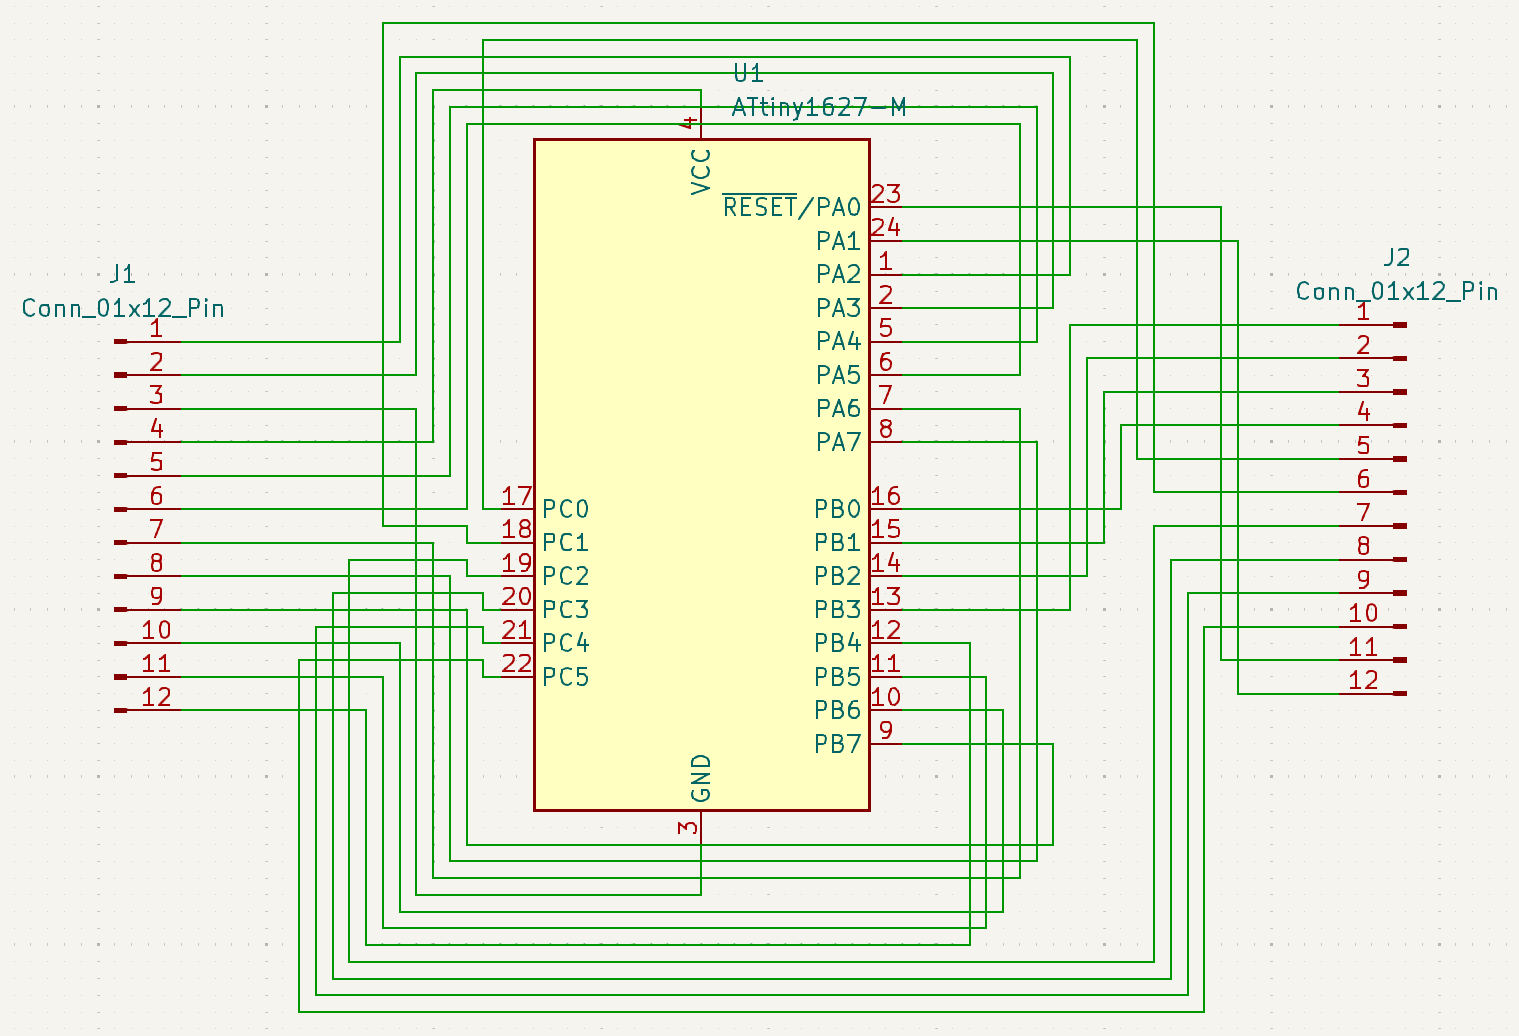
\includegraphics[width= \linewidth]{assets/breakout_schematic.png}
	\end{center}
	\begin{center}
		\label{picture:breakout2}
		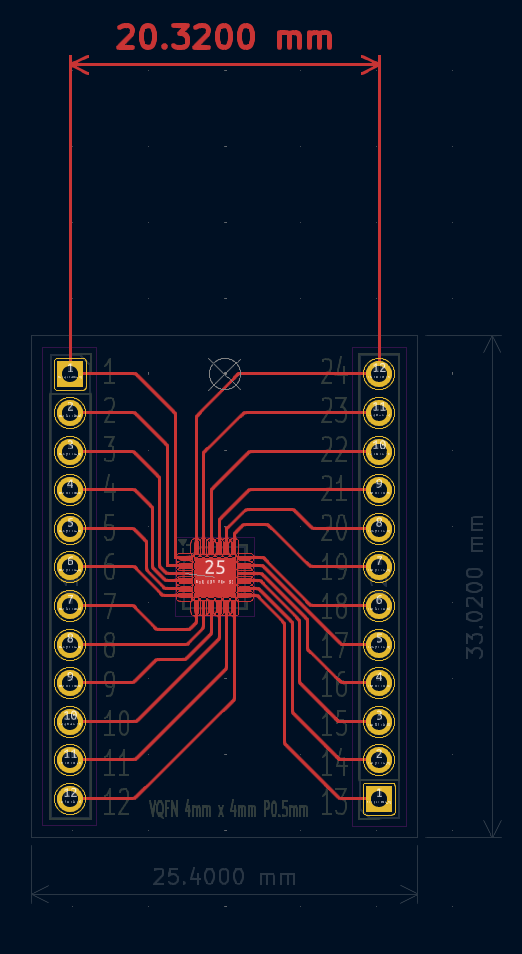
\includegraphics[width= \linewidth]{assets/breakout_pcb_schema.png}
	\end{center}
	\begin{center}
		\label{picture:breakout3}
		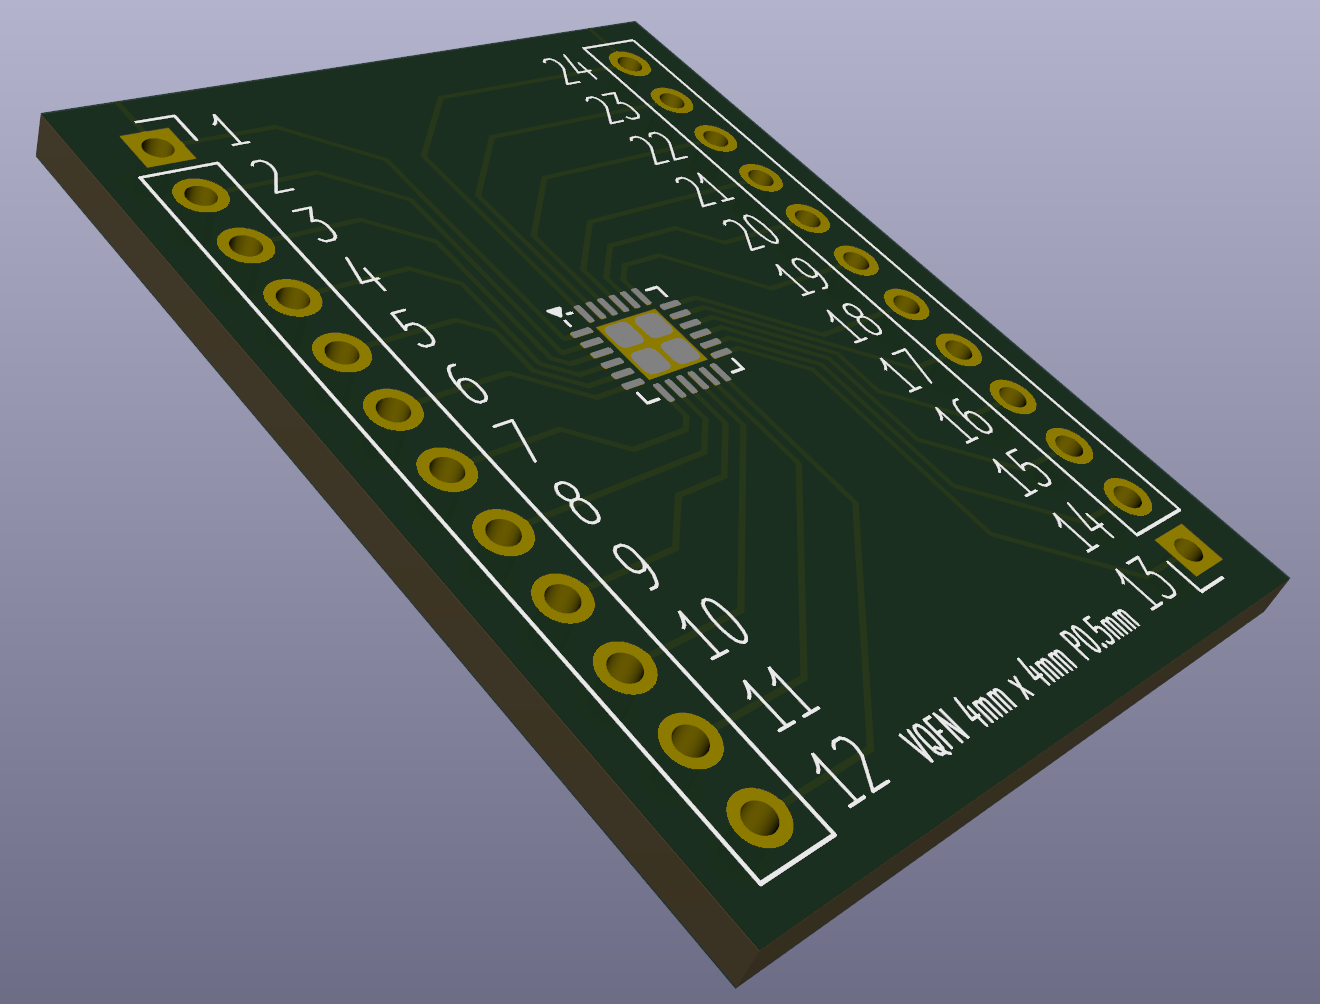
\includegraphics[width= \linewidth]{assets/breakout_pcb_3d.png}
	\end{center}
	
	\section{AUV Electronics Schematics}\label{appendix:auv_electronics_scematics}
	\subsection{AUV Schematic}\label{appendix:auv_schematic}
	\begin{center}
		\label{picture:auv_schematic}
		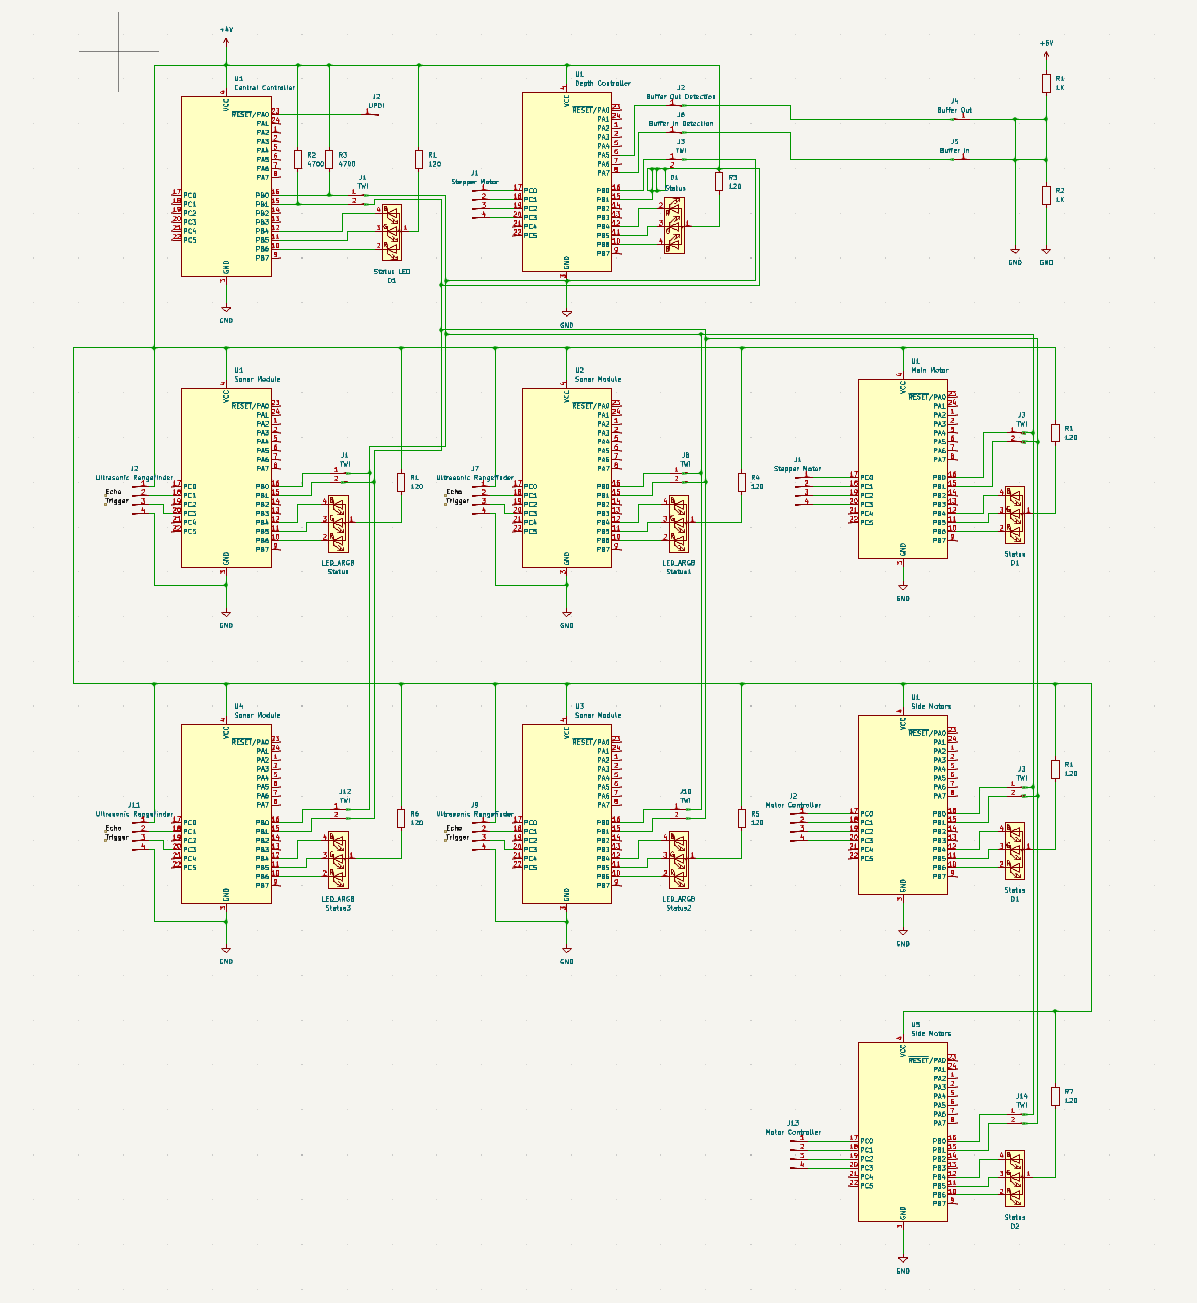
\includegraphics[width=\linewidth]{assets/AUVSchematic.png}
	\end{center}
	\subsection{Central Controller Schematic}\label{appendix:central_controller_schematic}
	\begin{center}
		\label{picture:central_controller_schematic}
		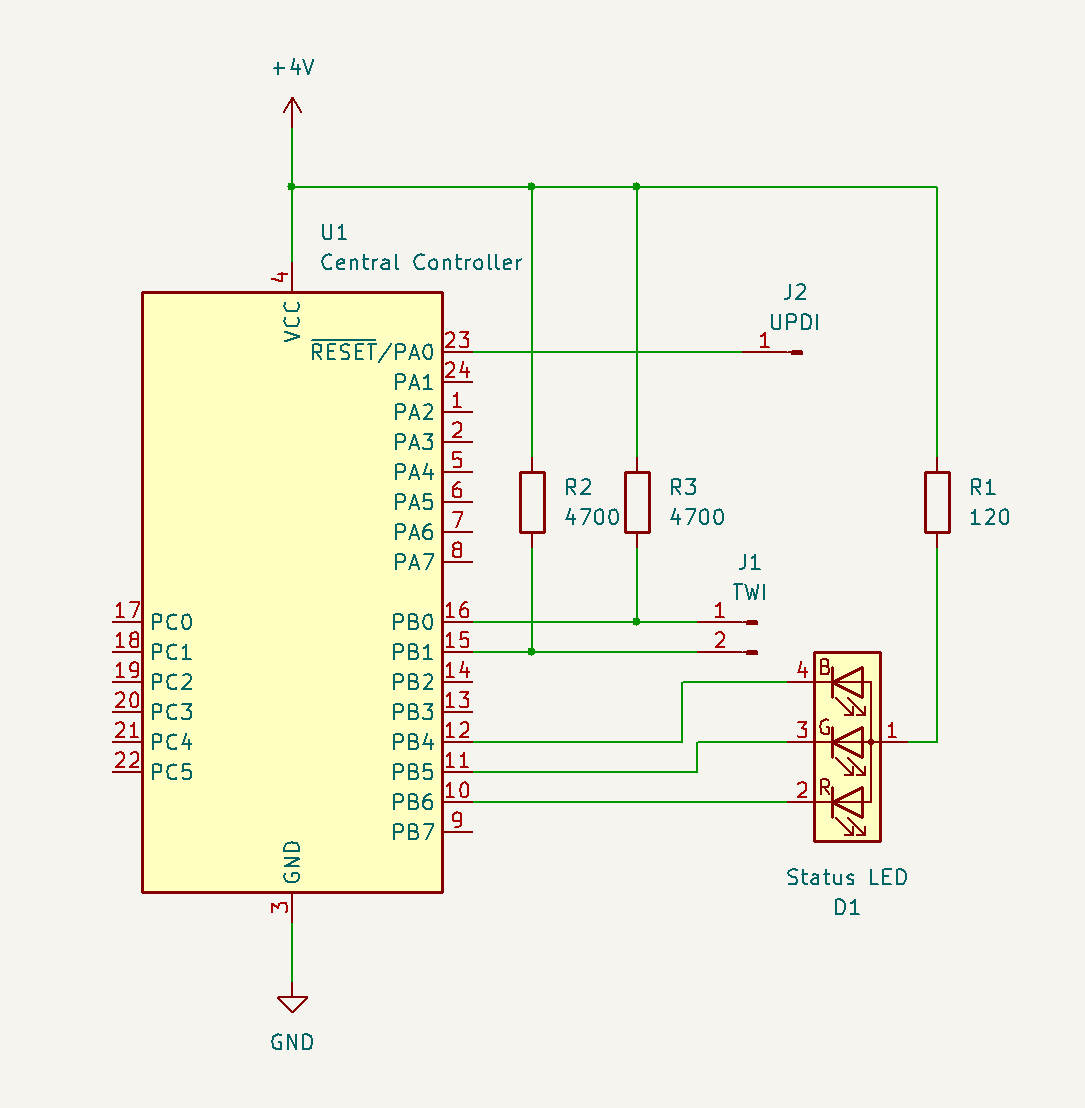
\includegraphics[width=\linewidth]{assets/CentralControllerSchematic.png}
	\end{center}
	\subsection{Depth Controller Schematic}\label{appendix:depth_controller_schematic}
	\begin{center}
		\label{picture:depth_controller_schematic}
		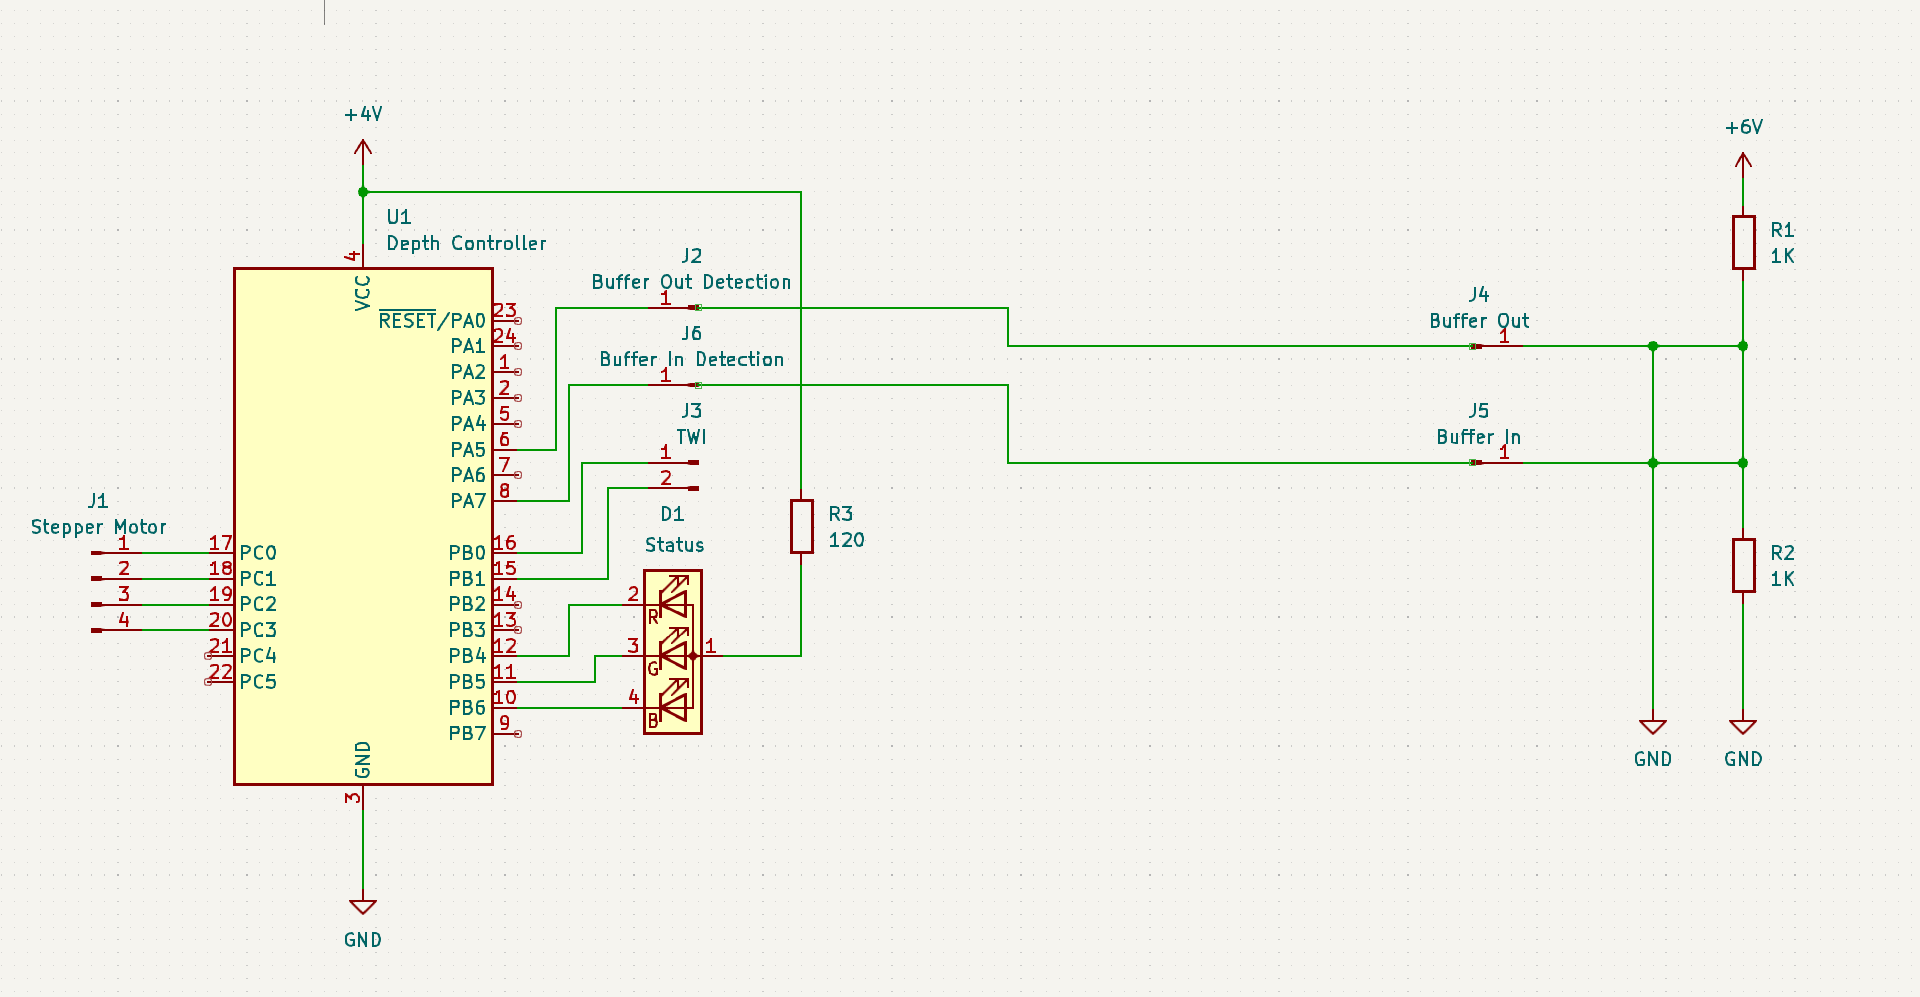
\includegraphics[width=\linewidth]{assets/DepthControllerSchematic.png}
	\end{center}
	\subsection{Sonar Module Schematic}\label{appendix:sonar_schematic}
	\begin{center}
		\label{picture:sonar_schematic}
		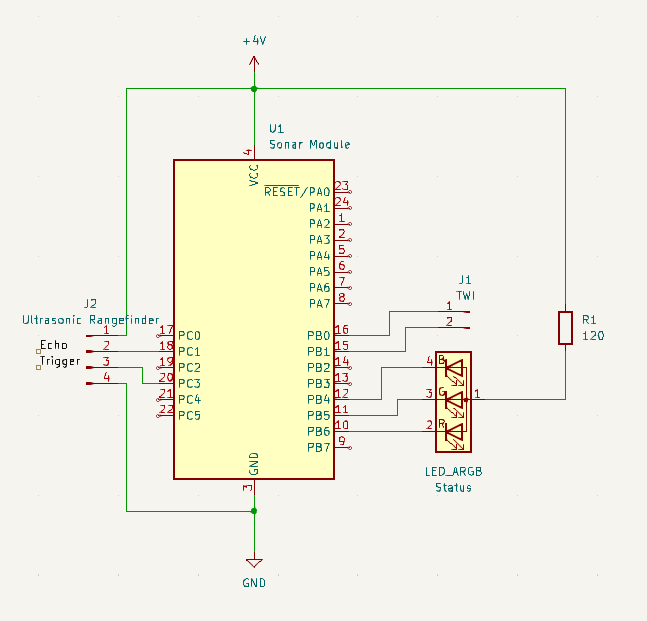
\includegraphics[width=\linewidth]{assets/SonarModuleSchematic.png}
	\end{center}
	\subsection{Main Motor Schematic}\label{appendix:main_motor_schematic}
	\begin{center}
		\label{picture:main_motor_schematic}
		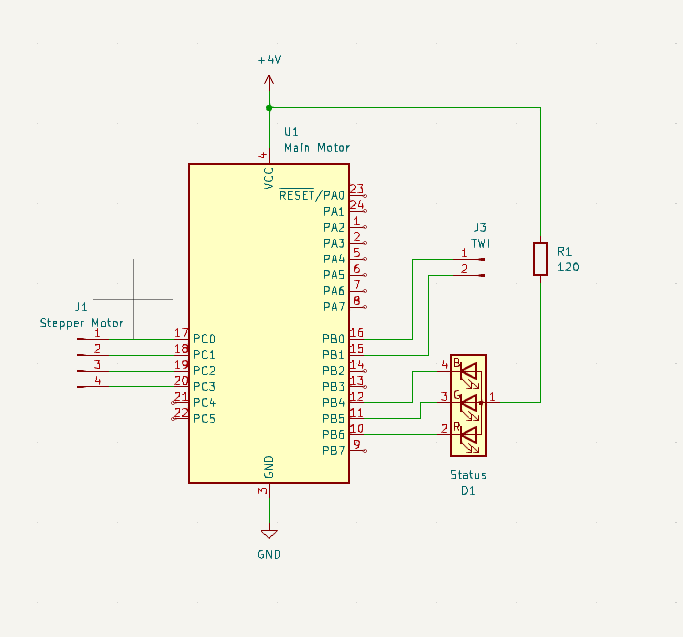
\includegraphics[width=\linewidth]{assets/MainMotorSchematic.png}
	\end{center}
	\subsection{Side Motor Schematic}\label{appendix:side_motor_schematic}
	\begin{center}
		\label{picture:side_motor_schematic}
		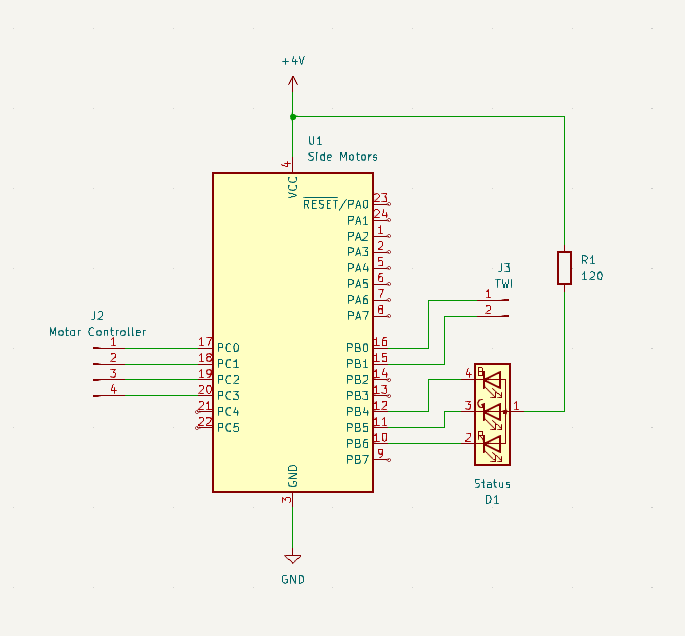
\includegraphics[width=\linewidth]{assets/SideMotorSchematic.png}
	\end{center}
	
	\section{Pseudocode}\label{appendix:pseudocode}
	\subsection{Central Controller}\label{appendix:central_controller_pseudocode}
	\begin{lstlisting}
		sonars = [lower, forward, left, right]
		sonarIndex
		depth = 255
		
		function getDepth: 
		return I2C.read(DEPTH_CONTROLLER_ADDR)
		
		setup:
		configure RTC for 1 second interrupts
		configure I2C as Host
		
		//Need to give the depth controller time to find its home position
		while(getDepth() != 1):
		delay(1000)
		
		dive(depth)
		
		//delay to give other modules time to properly initialise
		delay(2000);
		
		mainloop:
		//Does nothing
		
		function ping(sonar) {
			switch(sonar):
			case lower:
			//write operation to initialise the sonar module
			I2C.write(LOWER_SONAR_ADDR, PING_COMMAND)
			//wait for the sonar to finish then collect the results
			delay(250)
			return I2C.read(LOWER_SONAR_ADDR)
			case forward:
			//write operation to initialise the sonar module
			I2C.write(FORWARD_SONAR_ADDR, PING_COMMAND)
			//wait for the sonar to finish then collect the results
			delay(250)
			return I2C.read(FORWARD_SONAR_ADDR)
			case left:
			//write operation to initialise the sonar module
			I2C.write(LEFT_SONAR_ADDR, PING_COMMAND)
			//wait for the sonar to finish then collect the results
			delay(250)
			return I2C.read(LEFT_SONAR_ADDR)
			case right:
			//write operation to initialise the sonar module
			I2C.write(RIGHT_SONAR_ADDR, PING_COMMAND)
			//wait for the sonar to finish then collect the results
			delay(250)
			return I2C.read(RIGHT_SONAR_ADDR)
		}
		
		function handlePingResponse(sonar, distance):
			switch(sonar):
				case lower:
					if (distance < 10):
						depth -= 10
					else if (distance != 255):
						depth += 10
					if (depth > 255):
						depth = 255 
					if (depth < 0):
						depth = 0
					I2C.write(DEPTH_CONTROLLER_ADDR, depth)
				case forward:
					if (distance < 10):
						I2C.write(FORWARD_MOTOR_ADDR, STOP_COMMAND)
					else
						I2C.write(FORWARD_MOTOR_ADDR, FORWARD_COMMAND)
				case left:
					if (distance < 10):
						I2C.write(FORWARD_MOTOR_ADDR, STOP_COMMAND)
						I2C.write(LEFT_MOTOR_ADDR, TURN_COMMAND)
					else
						I2C.write(FORWARD_MOTOR_ADDR, FORWARD_COMMAND)
						I2C.write(LEFT_MOTOR_ADDR, STOP_COMMAND)
				case right:
					if (distance < 10):
						I2C.write(FORWARD_MOTOR_ADDR, STOP_COMMAND)
						I2C.write(RIGHT_MOTOR_ADDR, TURN_COMMAND)
					else
						I2C.write(FORWARD_MOTOR_ADDR, FORWARD_COMMAND)
						I2C.write(RIGHT_MOTOR_ADDR, STOP_COMMAND)
		
		//ISRs
		On_RTC_Interrupt:
			distance = ping(sonars[sonarIndex])
			handlePingResponse(sonars[sonarIndex], distance)
			sonarIndex += 1
			if (sonarIndex > 3):
				sonarIndex = 0
	\end{lstlisting}
	
	\subsection{Depth Controller}\label{appendix:depth_controller_pseudocode}
	\begin{lstlisting}
		depth = 255
		commandedPos = 0
		dir = IN
		
		setup:
			configure RTC for 1 second interrupts
			configure I2C as Client
			configure Pins for Stepper Motor
		
		function stepMotor(step):
			switch(step):
				case 0:
					Set pins to 1010
				case 1:
					Set pins to 1001
				case 2:
					Set pins to 0101
				case 3:
					Set pins to 0110
				case 4:
					Set pins to 0011
				case 5:
					Set pins to 1100
				case 6:
					Set pins to 0100
				case 7:
					Set pins to 1000
		
		function stopMotor():
			Set pins to 0000
		
		stepperStep = 0
		mainloop:
			if (depth != commandedPos):
				if (dir == OUT && plungerPos != 255):
					stepMotor(stepperStep)
					stepperStep -= 1
					//There are 8 possible steps (pin configurations) for the stepper
					//motor according to online resources/datasheet*
					
					//*Its a cheap stepper motor so datasheet is a very loose term.  
					if (stepperStep < 0):
					stepperStep = 7
					
				if (dir == IN && plungerPos != 0):
					stepMotor(stepperStep)
					stepperStep += 1
					if (stepperStep > 7):
					stepperStep = 0
			
			else:
				stopMotor()
		
		//ISRs
		On_RTC_Interrupt:
			if (depth != commandedPos):
				if (depth > commandedPos):
					dir = OUT
					commandedPos += 1
				else:
					dir = IN
					commandedPos -= 1
		
		On_I2C_RX:
			data = I2C.read()
			if (data > depth):
				dir = OUT
			else:
				dir = IN
			commandedPos = data
		
		On_I2C_TX:
			I2C.write(depth)
	\end{lstlisting}
	
	\subsection{Main Motor}\label{appendix:main_motor_pseudocode}
	\begin{lstlisting}
		dir = FORWARD
		
		setup:
			configure I2C as Client
			configure Pins for Stepper Motor
		
		function stepMotor(step):
			switch(step):
				case 0:
					Set pins to 1010
				case 1:
					Set pins to 1001
				case 2:
					Set pins to 0101
				case 3:
					Set pins to 0110
				case 4:
					Set pins to 0011
				case 5:
					Set pins to 1100
				case 6:
					Set pins to 0100
				case 7:
					Set pins to 1000
				
		function stopMotor():
			Set pins to 0000
		
		mainloop:
			if (dir == FORWARD):
				stepMotor(stepperStep)
				stepperStep += 1
				if (stepperStep > 7):
					stepperStep = 0
			else:
				stopMotor()
		
		// ISRs
		On_I2C_RX:
			dir = I2C.read()
	\end{lstlisting}
	
	\subsection{Sonar}\label{appendix:sonar_pseudocode}
	\begin{lstlisting}
		distance = 0
		
		setup:
			setup TCA to count to max value
			configure I2C as Client
			configure pins for sonar module
		
		mainloop:
			//Do nothing. wait for ISR
		
		function ping():
			//Pull trigger high and wait 10us
			TRIGGER_PIN = HIGH
			delay_us(10)
			TRIGGER_PIN = LOW
			TCA = ENABLE
			while (ECHO_PIN == HIGH):
				//Wait for echo pin to go low
		
			ticks = TCA.COUNT
			
			//Convert the TCA ticks to a time in uS
			clk = F_CPU/ 64
			time = ticks / clk
			
			sos = 148000
			//This should give us the distance in cm/uS
			distance = (time * sos) / 2
		
		// ISRs
		On_I2C_RX:
			distance = ping()
		
		On_I2C_TX:
			I2C.write(distance)
	\end{lstlisting}
	
	\subsection{Side Motor}\label{appendix:side_motor_pseudocode}
	\begin{lstlisting}
		setup:
			configure Pins for toy motor
			configure I2C as Client
		
		mainloop:
			//Do nothing. wait for ISR
		
		// ISRs
		On_I2C_RX:
			dir = I2C.read()
			if (dir == FORWARD):
				//Turn the motor on
				//twin motor driver. 
				//00 = off
				//01 = forward
				//10 = reverse
				//11 = brake
				MOTOR_PINS = 1010
			else:
				//Turn the motor off
				MOTOR_PIN = 0000
	\end{lstlisting}
	
	\section{Midterm $I^{2}C$}\label{appendix:midterm_i2c_code}
	\subsection{host.h}\label{appendix:midterm_i2c_host_h}
	\begin{lstlisting}
		#ifndef I2C_HOST_H
		#define I2C_HOST_H
		
		#ifndef F_CPU
		#define F_CPU 3333333UL
		#endif
		#include <avr/io.h>
		
		#define I2C_CHECK_START() (TWI_WIF_bm & TWI_CLKHOLD_bm) 
		#define I2C_CHECK_WRITE() (TWI_WIF_bm)
		#define I2C_CHECK_NACK() (TWI_WIF_bm & TWI_RXACK_bm)
		
		typedef struct {
			// Add any necessary fields here, if needed
		} I2C_Host;
		
		void I2C_Host_InitPins(void);
		
		void I2C_Host_InitI2C(void);
		
		uint8_t I2C_Host_CalcBaud(void);
		
		struct BAUD_TIMING_t{
			double T_LOW;
			double T_HIGH;
			double T_OF;
			double T_R;
		};
		
		double I2C_Host_CalcBaud_F_SCL(void);
		
		double I2C_Host_CalcBaud_BAUD(double);
		
		uint8_t I2C_Host_Start(uint8_t, uint8_t);
		
		void I2C_Host_WriteData(uint8_t);
		
		void I2C_Host_Stop(void);
		
		#endif // I2C_HOST_H
	\end{lstlisting}
	
	\subsection{host.c}\label{appendix:midterm_i2c_host_c}
	\begin{lstlisting}
		
		#include "I2C_Host.h"
		
		void I2C_Host_InitPins(void)
		{
			/**
			* Data sheet claims 1627 pins are the following:
			* 
			* PB0: SCL
			* PB1: SDA
			*/
			
			PORTB.DIR |= PIN0_bm | PIN1_bm;
			
			PORTB.PIN0CTRL |= PORT_PULLUPEN_bm;
			PORTB.PIN1CTRL |= PORT_PULLUPEN_bm;
		}
		
		void I2C_Host_InitI2C(void)
		{
			//Set the Master Baud Rate (Master defines baud for clients)
			//    TWI0.MBAUD = I2C_Host_CalcBaud();
			TWI0.MBAUD = 12;
			
			//Set the bus state to IDLE
			TWI0.MSTATUS |= TWI_BUSSTATE_IDLE_gc;
			
			//Enable Smart Mode. We need to set MCTRLB ACKACT set to ACK
			//Then MCTRLA SMEN (Smart Mode Enable) set to 1
			TWI0.MCTRLB = TWI_ACKACT_ACK_gc;
			
			//Enable the TWI
			TWI0.MCTRLA = TWI_SMEN_bm | TWI_ENABLE_bm;
		}
		
		uint8_t I2C_Host_CalcBaud(void)
		{
			double fSCL = I2C_Host_CalcBaud_F_SCL();
			double baud = I2C_Host_CalcBaud_BAUD(fSCL);
			return (uint8_t)(baud);
		}
		
		
		struct BAUD_TIMING_t BAUD_TIMING = {
			.T_LOW = 5.0e-6,
			.T_HIGH = 5.0e-6,
			.T_OF = 0,
			.T_R = 0
		}; //These values should produce time of 100000
		
		double I2C_Host_CalcBaud_F_SCL(void)
		{
			//f(SCL) = 1 / t_LOW + t_HIGH + t_OF + t_R
			/**
			* From the timing requirements we can infer that:
			* 
			* t_LOW:               MIN VALUE                   MAX VALUE
			*      @ <= 100kHZ     4.7us
			*      @ <= 400kHZ     1.3us
			*      @ <= 1MHz       0.5us
			* 
			* t_HIGH
			*      @ <= 100kHZ     4.0us
			*      @ <= 400kHZ     0.6us
			*      @ <= 1MHz       0.26us
			* 
			* t_OF
			*      @ <= 100kHZ     -                           250ns
			*      @ <= 400kHZ     20*(Vdd / 5.5)ns            250ns
			*      @ <= 1MHz       20*(Vdd / 5.5)ns            120ns
			* 
			* t_R
			*      @ <= 100kHZ     -                           1000ns
			*      @ <= 400kHZ     20ns                        300ns
			*      @ <= 1MHz       -                           120ns
			*/
			//init values in seconds
			
			double total = 5.0e-6 + 5.0e-6 + 0 + 0;
			double fSCL = 1.0 / total;
			return fSCL;
		}
		
		double I2C_Host_CalcBaud_BAUD(double fScl)
		{
			double baud = (F_CPU / 2*(fScl)) - (5 + ((F_CPU * BAUD_TIMING.T_R) / 2));
			return baud;
		}
		
		uint8_t I2C_Host_Start(uint8_t addr, uint8_t dir)
		{
			while ((TWI0.MSTATUS & TWI_BUSSTATE_gm) != TWI_BUSSTATE_IDLE_gc);
			//Write the address shifting one to the left. dir bit determines 
			//if Read(0x00) or write(0x01) operation
			TWI0.MADDR |= (addr << 1) | dir;
			
			//We only want to check the flags are high on write mode
			if (dir == 0x00)
			{
				//Check Interrupt Flags are high
				//        while(!(TWI0.MSTATUS & I2C_CHECK_START()));
				while (!(TWI0.MSTATUS & TWI_WIF_bm) || !(TWI0.MSTATUS & TWI_CLKHOLD_bm));
			}
			
			// all is good, return truthy
			return 0x01;
		}
		
		void I2C_Host_WriteData(uint8_t data)
		{
			//Writing to MData clears the WIF (Write Interrupt Flag)
			TWI0.MDATA = data;
			
			//Check for WIF
			while(!(TWI0.MSTATUS & I2C_CHECK_WRITE()))
			{
				if (TWI0.MSTATUS & I2C_CHECK_NACK())
				{
					//Error Handle. For now call stop?
					I2C_Host_Stop();
					return;
				}
			}
		}
		
		void I2C_Host_Stop(void)
		{
			//Send the Stop Command on MCTRLB
			TWI0.MCTRLB |= TWI_MCMD_STOP_gc;
		}
	\end{lstlisting}
	
	\subsection{client.h}\label{appendix:midterm_i2c_client_h}
	\begin{lstlisting}
		#ifndef I2C_CLIENT_H
		#define I2C_CLIENT_H
		
		#ifndef F_CPU
		#define F_CPU 3333333UL
		#endif
		#include <avr/io.h>
		#include <stddef.h>  // Include stddef.h for NULL
		#include <avr/interrupt.h>
		
		// Type definition for the receive callback function
		typedef void (*I2C_ReceiveCallback)(uint8_t data);
		
		// Function declarations
		void I2C_Client_InitPins(void);
		void I2C_Client_InitI2C(uint8_t address, I2C_ReceiveCallback callback);
		uint8_t I2C_Client_ReadData(void);
		void I2C_Client_WriteData(uint8_t data);
		
		#endif // I2C_CLIENT_H
	\end{lstlisting}
	
	\subsection{client.c}\label{appendix:midterm_i2c_client_c}
	\begin{lstlisting}
		#include "I2C_Client.h"
		
		// Global variable to store the receive callback function
		static I2C_ReceiveCallback receive_callback = NULL;
		
		// Initialize I2C pins
		void I2C_Client_InitPins(void)
		{
			// Set PB0 (SCL) and PB1 (SDA) as input
			PORTB.DIR &= ~(PIN0_bm | PIN1_bm);
		}
		
		// Initialize I2C in client mode
		void I2C_Client_InitI2C(uint8_t address, I2C_ReceiveCallback callback)
		{
			// Store the callback function
			receive_callback = callback;
			
			// Set the slave address
			TWI0.SADDR = address << 1 | 0x00; //| 0x01 respond to all addr. 
			
			// Enable the TWI and Smart Mode, clear collision and bus error flags
			TWI0.SCTRLA = TWI_ENABLE_bm | TWI_DIEN_bm | TWI_APIEN_bm | TWI_PIEN_bm;
			
			// Ensure the slave interface is enabled
			//    TWI0.SCTRLB = 0;
			sei();
		}
		
		// Read data from I2C
		uint8_t I2C_Client_ReadData(void)
		{
			// Wait for data to be received
			while (!(TWI0.SSTATUS & TWI_DIF_bm));
			
			// Check if data was received
			if (TWI0.SSTATUS & TWI_DIF_bm)
			{
				// Read and return the data
				return TWI0.SDATA;
			}
			
			// Return 0 if no data was received
			return 0;
		}
		
		// Write data to I2C
		void I2C_Client_WriteData(uint8_t data)
		{
			// Wait for the data register to be empty
			while (!(TWI0.SSTATUS & TWI_DIF_bm));
			
			// Write the data
			TWI0.SDATA = data;
			
			// Wait for the data to be transmitted
			while (!(TWI0.SSTATUS & TWI_DIF_bm));
		}
		
		// Interrupt Service Routine for I2C
		ISR(TWI0_TWIS_vect)
		{
			// Check if Address/Stop interrupt
			if (TWI0.SSTATUS & TWI_APIF_bm)
			{
				// Clear the interrupt flag
				TWI0.SSTATUS = TWI_APIF_bm;
				
				// Check if the address match
				if (TWI0.SSTATUS & TWI_AP_bm)
				{
					// Clear the address match flag
					TWI0.SSTATUS = TWI_AP_bm;
					TWI0.SCTRLB = TWI_SCMD_RESPONSE_gc;
				}
				else
				{
					// If not an address match, it must be a stop condition
					TWI0.SCTRLB = TWI_SCMD_COMPTRANS_gc;
				}
			}
			
			// Check if Data interrupt
			if (TWI0.SSTATUS & TWI_DIF_bm)
			{
				// Read the received data
				uint8_t received_data = TWI0.SDATA;
				
				//Call the receive callback if it's set
				if (receive_callback != NULL)
				{
					receive_callback(received_data);
				}
				
				// Clear the data interrupt flag
				TWI0.SSTATUS = TWI_DIF_bm;
			}
		}
	\end{lstlisting}
	\printbibliography
	
	\section{CWire Library}\label{appendix:cwire_library_code}
	\subsection{CWire.h}\label{appendix:cwire_h}
	\begin{lstlisting}
		#ifndef CWIRE_H
		#define	CWIRE_H
		
		#include<stdint.h>
		#include <avr/io.h>
		#include "Common.h"
		
		/* The Wire library unfortunately needs TWO buffers, one for TX, and one for RX. That means, multiply these
		* values by 2 to get the actual amount of RAM they take. You can see that on the smallest ram sizes, all but
		* the minuscule buffer we provide becomes prohibitive. 32b is a magic number because it's used on the stock
		* uno/etc cores, and many libraries rely on it implicitly.
		* | System RAM  | Buffer Size | Applies to
		* |-------------|-------------|----------------------------------------------------------------|
		* |  Under 256b |       2x16b | tinyAVR 0/1-series with 2k of flash (128b RAM)                 |
		* |   256-4095b |       2x32b | All other tinyAVR 0/1/2-series, and EA/DD-series with 8 or 16k |
		* |    >= 4096b |      2x130b | Dx, EA, and megaAVR 0-series with 32k flash or more            |
		*
		* On parts that get the reduced buffer size to fit in their limited RAM, the flash is also very small,
		* and while the enhanced wire library *will* fit on 2k parts, you have very little flash left for anything else.
		* and the practicality of using it there is limited.
		*/
		
		
		#ifndef ADD_READ_BIT
		#define ADD_READ_BIT(address)    (address | 0x01)
		#endif
		#ifndef ADD_WRITE_BIT
		#define ADD_WRITE_BIT(address)   (address & ~0x01)
		#endif
		
		#ifndef DEFAULT_FREQUENCY
		#define DEFAULT_FREQUENCY 100000
		#endif
		
		
		#if (!defined(TWI1) && defined(TWI_USING_WIRE1))
		// If pins for Wire1 are not defined, but TWI_USING_WIRE1 was defined in the boards.txt menu, throw an error. Used for 28-pin DA/DB parts
		#error "This part only provides a single Wire interface."
		#endif
		
		/* Instead of requiring changes to the library to switch between DxCore and megaTinyCore, we can check
		* if the part supports dual mode. Goal is that the identical library can be used on both, so updates
		* in one can be propagated to the other by just copying files.
		*/
		#if ((defined(TWI0_DUALCTRL) && !defined(TWI_USING_WIRE1)) || (defined(TWI1_DUALCTRL) && defined(TWI_USING_WIRE1)))
		#define TWI_DUALCTRL   // This identifies if the device supports dual mode, where slave pins are different from the master pins
		#endif
		
		
		#if defined(__AVR_ATtiny202__) || defined(__AVR_ATtiny202__)
		#if defined(TWI_MANDS)  // 202 and 402 do not support independent master and slave.
		// #undef TWI_MANDS
		#error "Master + Slave mode is not supported on the 202 or 402."
		// If a user enables master + slave mode on a part where we know it won't we should error
		// so that they know what's wrong instead of silently disobeying
		#endif
		#endif
		
		
		// WIRE_HAS_END means Wire has end(), which almost all implementations do.
		#ifndef WIRE_HAS_END
		#define WIRE_HAS_END 1
		#endif
		
		// These can be used to write clearer code when using the three-argument begin()
		// An alternate address is specified by leftshifting and setting the low bit to 1
		#define WIRE_ALT_ADDRESS(addr) ((addr << 1) | 0x01)
		// While a mask is specified by leftshifting the mask, and leaving low bit 0.
		#define WIRE_ADDRESS_MASK(mask) (mask << 1)
		
		#define WIRE_SDA_HOLD_OFF 0
		#define WIRE_SDA_HOLD_50  1
		#define WIRE_SDA_HOLD_300 2
		#define WIRE_SDA_HOLD_500 3
		
		#define WIRE_SDA_SETUP_4  0
		#define WIRE_SDA_SETUP_8  1
		
		#define WIRE_I2C_LEVELS  0
		#define WIRE_SMBUS_LEVELS  1
		
		
		
		#if !defined(TWI_BUFFER_LENGTH)       // we need a Buffer size
		#if defined(BUFFER_LENGTH) && (BUFFER_LENGTH != 32)   // Backwards Compatibility: someone needs a non-default size
		#define TWI_BUFFER_LENGTH BUFFER_LENGTH             // Apply it.
		#warning "It seems like BUFFER_LENGTH was used to change the default Wire Buffer Size."
		#warning "The define was renamed to TWI_BUFFER_LENGTH to reduce ambiguity."
		#warning "TWI_BUFFER_LENGTH was set to BUFFER_LENGTH." // defining TWI_BUFFER_LENGTH= will remove the warnings
		
		#else                               // BUFFER_LENGTH was not messed with, go with our defaults
		#if (RAMSIZE < 256)
		#define TWI_BUFFER_LENGTH 16
		#elif (RAMSIZE < 4096)
		#define TWI_BUFFER_LENGTH 32
		#else
		#define TWI_BUFFER_LENGTH 130
		#endif
		#endif
		#endif
		
		// In the case someone wants to use custom 255+ buffer sizes, define TWI_16BIT_BUFFER
		#if (TWI_BUFFER_LENGTH > 255) || defined(TWI_16BIT_BUFFER)
		typedef uint16_t twi_buf_index_t;
		#else
		typedef uint8_t  twi_buf_index_t;
		#endif
		
		
		#define  TWI_TIMEOUT_ENABLE       // Enabled by default, might be disabled for debugging or other reasons
		#define  TWI_ERROR_ENABLED        // Enabled by default, TWI Master Write error functionality
		#define  TWI_READ_ERROR_ENABLED   // Enabled on Master Read too
		//#define DISABLE_NEW_ERRORS      // Disables the new error codes and returns TWI_ERR_UNDEFINED instead.
		
		// Errors from Arduino documentation:
		#define  TWI_ERR_SUCCESS         0x00  // Default
		#define  TWI_ERR_DATA_TOO_LONG   0x01  // Not used here; data too long to fit in TX buffer
		#define  TWI_ERR_ACK_ADR         0x02  // Address was NACKed on Master write
		#define  TWI_ERR_ACK_DAT         0x03  // Data was NACKed on Master write
		#define  TWI_ERR_UNDEFINED       0x04  // Software can't tell error source
		#define  TWI_ERR_TIMEOUT         0x05  // TWI Timed out on data rx/tx
		
		// Errors that are made to help finding errors on TWI lines. Only here to give a suggestion of where to look - these may not always be reported accurately.
		#if !defined(DISABLE_NEW_ERRORS)
		#define  TWI_ERR_UNINIT        0x10  // TWI was in bad state when function was called.
		#define  TWI_ERR_PULLUP        0x11  // Likely problem with pull-ups
		#define  TWI_ERR_BUS_ARB       0x12  // Bus error and/or Arbitration lost
		#define  TWI_ERR_BUF_OVERFLOW  0x13  // Buffer overflow on master read
		#define  TWI_ERR_CLKHLD        0x14  // Something's holding the clock
		#else
		// DISABLE_NEW_ERRORS can be used to more completely emulate the old error reporting behavior; this should rarely be needed.
		#define  TWI_ERR_UNINIT        TWI_ERR_UNDEFINED  // TWI was in bad state when method was called.
		#define  TWI_ERR_PULLUP        TWI_ERR_UNDEFINED  // Likely problem with pull-ups
		#define  TWI_ERR_BUS_ARB       TWI_ERR_UNDEFINED  // Bus error and/or Arbitration lost
		#define  TWI_ERR_BUF_OVERFLOW  TWI_ERR_UNDEFINED  // Buffer overflow on master read
		#define  TWI_ERR_CLKHLD        TWI_ERR_UNDEFINED  // Something's holding the clock
		#endif
		
		#if defined(TWI_ERROR_ENABLED)
		#define TWI_ERROR_VAR    twi_error
		#define TWI_INIT_ERROR   uint8_t TWI_ERROR_VAR = TWI_ERR_SUCCESS
		#define TWI_GET_ERROR    TWI_ERROR_VAR
		#define TWI_CHK_ERROR(x) TWI_ERROR_VAR == x
		#define TWI_SET_ERROR(x) TWI_ERROR_VAR = x
		#else
		#define TWI_ERROR_VAR     {}
		#define TWI_INIT_ERROR    {}
		#define TWI_GET_ERROR     {0}
		#define TWI_CHK_ERROR(x)  (true)
		#define TWI_SET_ERROR(x)  {}
		#endif
		
		#if defined(TWI_READ_ERROR_ENABLED) && defined(TWI_ERROR_ENABLED)
		#define TWIR_ERROR_VAR        twiR_error
		#define TWIR_INIT_ERROR       uint8_t TWIR_ERROR_VAR = TWI_ERR_SUCCESS
		#define TWIR_GET_ERROR        TWIR_ERROR_VAR
		#define TWIR_CHK_ERROR(x)     TWIR_ERROR_VAR == x
		#define TWIR_SET_ERROR(x)     TWIR_ERROR_VAR = x
		
		// #define TWI_SET_EXT_ERROR(x)  TWI_ERROR_VAR = x
		#else
		#define TWIR_ERROR_VAR        {}
		#define TWIR_INIT_ERROR       {}
		#define TWIR_GET_ERROR        {0}
		#define TWIR_CHK_ERROR(x)     (true)
		#define TWIR_SET_ERROR(x)     {}
		
		// #define TWI_SET_EXT_ERROR(x)  {}
		#endif
		
		typedef struct {
			u8 _toggleStreamFn;
			u8 _hostEnabled;
			u8 _clientEnabled;
			u8 _hostDataSent;
			u8 _reserved;
		} twiDataBools;
		
		typedef struct {
			TWI_t *_module;
			u8 client_irq_mask;
			u8 _hostBuffer[TWI_BUFFER_LENGTH];
			u8 _clientBuffer[TWI_BUFFER_LENGTH];
			u8 _clientAddress;
			twi_buf_index_t _bytesToReadWrite;
			twi_buf_index_t _bytesReadWritten;
			twi_buf_index_t _bytesTransmittedS;
			twiDataBools _bools;
			void (*user_onReceive)(u8);
			void (*user_onRequest)(void);
		} TwoWire;
		
		#if (TWI_BUFFER_LENGTH > 255) || defined(TWI_16BIT_BUFFER)
		typedef uint16_t twi_buf_index_t;
		#else
		typedef uint8_t  twi_buf_index_t;
		#endif
		
		u8 MasterCalcBaud(u32 freq);
		
		void TwoWire_init(TwoWire *self, TWI_t *twi_module);
		u8 TwoWire_pins(TwoWire *self, u8 sda, u8 scl);
		//u8 TwoWire_swap(TwoWire *self, u8 state);
		//u8 TwoWire_swapModule(TwoWire *self, TWI_t *twi_module);
		void TwoWire_usePullups(TwoWire *self);
		u8 TwoWire_setClock(TwoWire *self, u32 freq);
		
		// Master
		void TwoWire_Master_begin(TwoWire *self);
		void TwoWire_endMaster(TwoWire *self);
		void TwoWire_beginTransmission(TwoWire *self, u8 addr);
		u8 TwoWire_endTransmission(TwoWire *self, u8 sendStop);
		twi_buf_index_t TwoWire_requestFrom(TwoWire *self, u8 addr, twi_buf_index_t qty, u8 sendStop);
		u8 TwoWire_masterTransmit(TwoWire *self, twi_buf_index_t *length, u8 *buff, u8 addr, u8 sendStop);
		u8 TwoWire_masterReceive(TwoWire *self, u16 *length, u8 *buff, u8 addr, u8 sendStop);
		
		// Slave
		void TwoWire_Slave_begin(TwoWire *self, u8 addr, u8 bc, u8 sec_addr);
		void TwoWire_endSlave(TwoWire *self);
		u8 TwoWire_getIncomingAddress(TwoWire *self);
		twi_buf_index_t TwoWire_getBytesRead(TwoWire *self);
		u8 TwoWire_slaveTransactionOpen(TwoWire *self);
		u8 TwoWire_checkPinLevels(TwoWire *self);
		//void TwoWire_selectSlaveBuffer(TwoWire *self);
		//void TwoWire_deselectSlaveBuffer(TwoWire *self);
		void TwoWire_HandleSlaveIRQ(TwoWire *wire_s);
		
		// Data handling
		u8 TwoWire_write(TwoWire *self, u8 data);
		u8 TwoWire_writeBytes(TwoWire *self, const u8 *data, u16 length);
		//u8 TwoWire_write(TwoWire *self, u8 data);
		//u8 TwoWire_writeBytes(TwoWire *self, const u8 *data, u16 length);
		//u8 TwoWire_writeUInt8(TwoWire *self, u8 n);
		//u8 TwoWire_writeUInt32(TwoWire *self, u32 n);
		//u8 TwoWire_writeInt(TwoWire *self, int n);
		int TwoWire_available(TwoWire *self);
		int TwoWire_read(TwoWire *self);
		int TwoWire_peek(TwoWire *self);
		
		void TwoWire_onReceive(TwoWire *self, void (*)(u8));
		void TwoWire_onRequest(TwoWire *self, void (*)(void));
		
		// Common
		void TwoWire_end(TwoWire *self);
		void TwoWire_flush(TwoWire *self);
		//u8 TwoWire_specialConfig(TwoWire *self, u8 smbus1v1, u8 longsetup, u8 sda_hold, u8 smbus1v1_dual, u8 sda_hold_dual);
		//void TwoWire_enableDualMode(TwoWire *self, u8 fmp_enable);
		
		#endif	/* CWIRE_H */
	\end{lstlisting}
	
	\subsection{CWire.c}\label{appendix:cwire_c}
	\begin{lstlisting}
		#include <stdlib.h>
		//#include <string.h>
		//#include <inttypes.h>
		#include <avr/interrupt.h>
		
		#ifndef F_CPU
		#define F_CPU 3333333UL
		#endif
		
		#include "CWire.h"
		
		#ifndef TWI0
		#define TWI0
		#endif
		
		#include "twi_pins.h"
		
		volatile u8 sleepStack = 0;
		
		void pauseDeepSleep(u8 moduelAddr);
		void restoreSleep(u8 moduelAddr);
		
		TwoWire* twi0_wire;
		
		#define TWI_BAUD(freq, t_rise) ((F_CPU / freq) / 2) - (5 + (((F_CPU / 1000000) * t_rise) / 2000))
		u8 MasterCalcBaud(u32 freq) {
			i16 baud;
			if (freq >= 600000) {          // assuming 1.5kOhm
				baud = TWI_BAUD(freq, 250);
			} else if (freq >= 400000) {   // assuming 2.2kOhm
				baud = TWI_BAUD(freq, 400);
			} else {                            // assuming 4.7kOhm
				baud = TWI_BAUD(freq, 600);
			}
			
			const u8 baudlimit = 0;
			
			if (baud < baudlimit) {
				return baudlimit;
			} else if (baud > 255) {
				return 255;
			}
			
			return (u8)baud;
		}
		
		void TwoWire_init(TwoWire *self, TWI_t *twi_module) {
			self->_module = twi_module;
			twi0_wire = self;
		}
		
		u8 TwoWire_pins(TwoWire *self, u8 sda, u8 scl) {
			return TWI0_Pins(sda, scl);
		}
		
		void TwoWire_usePullups(TwoWire *self) {
			TWI0_usePullups();
		}
		
		u8 TwoWire_setClock(TwoWire *self, u32 freq) {
			TWI_t* module = self->_module;
			if (__builtin_constant_p(freq)) {
				if ((freq < 1000) || (freq > 15000000)) {
					return 1;
				}
			} else {
				if (freq < 1000) {
					return 1;
				}
			}
			if (self->_bools._hostEnabled == 1) {
				u8 newBaud = MasterCalcBaud(freq);
				u8 oldBaud = module->MCTRLA;
				if (newBaud != oldBaud) {
					u8 restore = module->MCTRLA;
					module->MCTRLA = 0;
					module->MBAUD = newBaud;
					if (freq > 400000) {
						module->CTRLA |= TWI_FMPEN_bm;
					} else {
						module->CTRLA &= ~TWI_FMPEN_bm;
					}
					module->MCTRLA = restore;
					if (restore & TWI_ENABLE_bm) {
						module->MSTATUS = TWI_BUSSTATE_IDLE_gc;
					}
				}
				return 0;
			}
			return 1;
		}
		
		//Master
		void TwoWire_Master_begin(TwoWire *self) {
			TWI0_ClearPins();
			
			self->_bools._hostEnabled = 1;
			TWI_t* module = self->_module;
			module->MCTRLA = TWI_ENABLE_bm;
			module->MSTATUS = TWI_BUSSTATE_IDLE_gc;
			
			TwoWire_setClock(self, DEFAULT_FREQUENCY);
		}
		
		void TwoWire_endMaster(TwoWire *self) {
			if (true == self->_bools._hostEnabled) {
				self->_module->MCTRLA = 0x00;
				self->_module->MBAUD  = 0x00;
				self->_bools._hostEnabled  = 0x00;
			}
		}
		
		void TwoWire_beginTransmission(TwoWire *self, u8 addr) {
			if (__builtin_constant_p(addr) > 0x7F) {
				badArg("Supplied address seems to be 8 bit. Only 7 bit addresses are supported");
				return;
			}
			if (self->_bools._hostEnabled) {
				self->_clientAddress = addr << 1;
				self->_bytesToReadWrite = 0;
				self->_bytesReadWritten = 0;
			}
		}
		u8 TwoWire_endTransmission(TwoWire *self, u8 sendStop) {
			return TwoWire_masterTransmit(self, &self->_bytesToReadWrite, self->_hostBuffer, self->_clientAddress, sendStop);
		}
		
		twi_buf_index_t TwoWire_requestFrom(TwoWire *self, u8 addr, twi_buf_index_t qty, u8 sendStop) {
			if (__builtin_constant_p(qty)) {
				if (qty > TWI_BUFFER_LENGTH) {
					badArg("requestFrom requests more bytes than buffer space");
				}
			}
			if (qty >= TWI_BUFFER_LENGTH) {
				qty = TWI_BUFFER_LENGTH;
			}
			
			self->_clientAddress = addr << 1;
			self->_bytesToReadWrite = qty;
			self->_bytesReadWritten = 0;
			
			return TwoWire_masterReceive(self, &self->_bytesToReadWrite, self->_hostBuffer, self->_clientAddress, sendStop);
		}
		
		u8 TwoWire_masterTransmit(TwoWire *self, twi_buf_index_t *length, u8 *buff, u8 addr, u8 sendStop) {
			TWI_t* module = self->_module;
			__asm__ __volatile__("\n\t" : "+z"(module));
			
			TWI_INIT_ERROR;
			u8 currentSM;
			u8 currentStatus;
			u8 stat = 0;
			
			u16 dataToWrite = *length;
			#if defined (TWI_TIMEOUT_ENABLE)
			u16 timeout = (F_CPU/1000);
			#endif
			
			if ((module->MCTRLA & TWI_ENABLE_bm) == 0x00) {
				return TWI_ERR_UNINIT;
			}
			
			while (1) {
				currentStatus = module->MSTATUS;
				currentSM = currentStatus & TWI_BUSSTATE_gm;
				
				if (currentSM == TWI_BUSSTATE_UNKNOWN_gc) {
					return TWI_ERR_UNINIT;
				}
				
				#if defined (TWI_TIMEOUT_ENABLE)
				if (--timeout == 0) {
					if (currentSM == TWI_BUSSTATE_OWNER_gc) {
						TWI_SET_ERROR(TWI_ERR_TIMEOUT);
					} else if (currentSM == TWI_BUSSTATE_IDLE_gc) {
						TWI_SET_ERROR(TWI_ERR_PULLUP);
					} else {
						TWI_SET_ERROR(TWI_ERR_UNDEFINED);
					}
					break;
				}
				#endif
				
				if (currentStatus & TWI_ARBLOST_bm) {
					TWI_SET_ERROR(TWI_ERR_BUS_ARB);
					break;
				}
				
				if (currentSM != TWI_BUSSTATE_BUSY_gc) {
					if (stat == 0x00) {
						module->MADDR = ADD_WRITE_BIT(addr);
						stat |= 0x01;
						#if defined (TWI_TIMEOUT_ENABLE)
						timeout = (F_CPU/1000);
						#endif
					} else {
						if (currentStatus & TWI_WIF_bm) {
							if (currentStatus & TWI_RXACK_bm) {
								if (stat & 0x02) {
									if (dataToWrite != 0) {
										TWI_SET_ERROR(TWI_ERR_ACK_DAT);
									} 
								} else {
									TWI_SET_ERROR(TWI_ERR_ACK_ADR);
								}
								break;
							} else {
								if (dataToWrite != 0) {
									module->MDATA = *buff;
									buff++;
									dataToWrite--;
									stat |= 0x02;
									#if defined (TWI_TIMEOUT_ENABLE) 
									timeout = (F_CPU/1000);
									#endif
								} else {
									break;
								}
							}
						}
					}
				}
			}
			
			*length -= dataToWrite;
			if ((sendStop != 0) || (TWI_ERR_SUCCESS != TWI_GET_ERROR)) {
				module->MCTRLB = TWI_MCMD_STOP_gc;
			}
			return TWI_GET_ERROR;
		}
		
		u8 TwoWire_masterReceive(TwoWire *self, u16 *length, u8 *buff, u8 addr, u8 sendStop) {
			TWI_t *module = self->_module;
			__asm__ __volatile__("\n\t" : "+z"(module));
			
			TWIR_INIT_ERROR;
			u16 dataToRead = *length;
			
			u8 currentSM;
			u8 currentStatus;
			u8 state = 0;
			#if defined (TWI_TIMEOUT_ENABLE)
			u16 timeout = (F_CPU/1000);
			#endif
			
			while(1) {
				currentStatus = module->MSTATUS;
				currentSM = currentStatus & TWI_BUSSTATE_gm;
				
				if (currentSM == TWI_BUSSTATE_UNKNOWN_gc) {
					TWIR_SET_ERROR(TWI_ERR_UNINIT);
					break;
				}
				
				#if defined (TWI_TIMEOUT_ENABLE)
				if (--timeout == 0) {
					if (currentSM == TWI_BUSSTATE_OWNER_gc) {
						TWIR_SET_ERROR(TWI_ERR_TIMEOUT);
					} else if (currentSM == TWI_BUSSTATE_IDLE_gc) {
						TWIR_SET_ERROR(TWI_ERR_PULLUP);
					} else {
						TWIR_SET_ERROR(TWI_ERR_UNDEFINED);
					}
					break;
				}
				#endif
				
				if (currentStatus & TWI_ARBLOST_bm) {
					TWIR_SET_ERROR(TWI_ERR_BUS_ARB);
					break;
				}
				
				if (currentSM != TWI_BUSSTATE_BUSY_gc) {
					if (state == 0x00) {
						module->MADDR = ADD_READ_BIT(addr);
						state |= 0x01;
						#if defined (TWI_TIMEOUT_ENABLE)
						timeout = (F_CPU / 1000);
						#endif
					} else {
						if (currentStatus & TWI_WIF_bm) {
							TWIR_SET_ERROR(TWI_ERR_ACK_ADR);
							module->MCTRLB = TWI_MCMD_STOP_gc;
							break;
						} else if (currentStatus & TWI_RIF_bm) {
							*buff = module->MDATA;
							buff++;
							#if defined (TWI_TIMEOUT_ENABLE)
							timeout = (F_CPU / 1000);
							#endif
							if (--dataToRead != 0) {
								module->MCTRLB = TWI_MCMD_RECVTRANS_gc;
							} else {
								if (sendStop != 0) {
									module->MCTRLB = TWI_ACKACT_bm | TWI_MCMD_STOP_gc;
								} else {
									module->MCTRLB = TWI_ACKACT_bm;
								}
								break;
							}
						}
					}
				}
			}
			*length -= dataToRead;
			return TWIR_GET_ERROR;
		}
		
		// Slave
		void TwoWire_Slave_begin(TwoWire *self, u8 addr, u8 bc, u8 sec_addr) {
			if (__builtin_constant_p(addr)) {
				if (addr > 0x7F) {
					badArg("TWI addresses must be supplied in 7-bit format");
					return;
				}
			}
			
			#if defined(TWI_MANDS)
			if (self->_bools._clientEnabled == 1) {
				return;
			}
			#else
			if ((self->_bools._hostEnabled | self->_bools._clientEnabled) == 1) {
				return;
			}
			#endif
			
			TWI0_ClearPins();
			
			self->_bools._clientEnabled = 1;
			self->client_irq_mask= TWI_COLL_bm;
			TWI_t* module = self->_module;
			module->SADDR = (addr << 1) | bc; //broadcast
			module->SADDRMASK = sec_addr;
			module->SCTRLA = TWI_DIEN_bm | TWI_APIEN_bm | TWI_PIEN_bm | TWI_ENABLE_bm;
		}
		
		void TwoWire_endSlave(TwoWire *self) {
			if (self->_bools._clientEnabled == 1) {
				self->_module->SADDR = 0x00;
				self->_module->SCTRLA = 0x00;
				self->_module->SADDRMASK = 0x00;
				self->_bools._clientEnabled = 0x00;
			}
		}
		
		u8 TwoWire_getIncomingAddress(TwoWire *self) {
			#if defined (TWI_MANDS) 
			return self->_incomingAddress;
			#else
			return self->_clientAddress;
			#endif
		}
		
		twi_buf_index_t TwoWire_getBytesRead(TwoWire *self) {
			twi_buf_index_t num = self->_bytesTransmittedS;
			self->_bytesTransmittedS = 0;
			return num;
		}
		
		u8 TwoWire_slaveTransactionOpen(TwoWire *self) {
			u8 status = self->_module->SSTATUS;
			if (!(status & TWI_AP_bm)) {
				return 0;
			}
			if (status & TWI_DIR_bm) {
				return 2;
			}
			return 1;
		}
		
		u8 TwoWire_checkPinLevels(TwoWire *self) {
			return TWI0_checkPinLevel();
		}
		
		void TwoWire_onReceive(TwoWire *self, void (*function)(u8)) {
			self->user_onReceive = function;
		}
		
		void TwoWire_onRequest(TwoWire *self, void (*function)(void)) {
			self->user_onRequest = function;
		}
		
		ISR(TWI0_TWIS_vect) {
			TwoWire_HandleSlaveIRQ(twi0_wire);
		}
		
		void TwoWire_HandleSlaveIRQ(TwoWire *wire_s) {
			if (wire_s == NULL) {
				return;
			}
			
			u8 *address,  *buffer;
			twi_buf_index_t *head, *tail;
			#if defined(TWI_MANDS)
			address = &(wire_s->_incomingAddress);
			head    = &(wire_s->_bytesToReadWriteS);
			tail    = &(wire_s->_bytesReadWrittenS);
			buffer  =   wire_s->_clientBuffer;
			#else
			address = &(wire_s->_clientAddress);
			head    = &(wire_s->_bytesToReadWrite);
			tail    = &(wire_s->_bytesReadWritten);
			buffer  =   wire_s->_hostBuffer;
			#endif
			
			#if defined(TWI_MANDS)
			wire_s->_bools._toggleStreamFn = 0x01;
			#endif
			
			u8 action = 0;
			u8 clientStatus = wire_s->_module->SSTATUS;
			
			
			if (clientStatus & TWI_APIF_bm) {   // Address/Stop Bit set
				if (wire_s->_bools._hostDataSent != 0) { // At this point, we have either a START, REPSTART or a STOP
					wire_s->_bools._hostDataSent = 0x00;
					if (wire_s->user_onReceive != NULL) {   // only if the last APIF was a Master Write,
						wire_s->user_onReceive((*head));      // we notify the sketch about new Data
					}
				}
				
				if (clientStatus & TWI_AP_bm) {     // Address bit set
					if ((*head) == 0) {                 // only if there was no data (START)
						pauseDeepSleep((u8)((u16)wire_s->_module));  // Only START can wake from deep sleep, change to IDLE
					}
					(*head) = 0;
					(*tail) = 0;
					(*address) = wire_s->_module->SDATA;  // read address from data register
					if (clientStatus & TWI_DIR_bm) {      // Master is reading
						if (wire_s->user_onRequest != NULL) {
							wire_s->user_onRequest();
						}
						if ((*head) == 0) {                     // If no data to transmit, send NACK
							action = TWI_ACKACT_bm | TWI_SCMD_COMPTRANS_gc;  // NACK + "Wait for any Start (S/Sr) condition"
						} else {
							action = TWI_SCMD_RESPONSE_gc;        // "Execute Acknowledge Action succeeded by reception of next byte"
						}
					} else {                          // Master is writing
						wire_s->_bools._hostDataSent = 0x01;
						action = TWI_SCMD_RESPONSE_gc;  // "Execute Acknowledge Action succeeded by slave data interrupt"
					}
				} else {                          // Stop bit set
					restoreSleep((u8)((u16)wire_s->_module));
					(*head) = 0;
					(*tail) = 0;
					action = TWI_SCMD_COMPTRANS_gc;  // "Wait for any Start (S/Sr) condition"
				}
			} else if (clientStatus & TWI_DIF_bm) { // Data bit set
				if (clientStatus & TWI_DIR_bm) {        // Master is reading
					if (clientStatus & wire_s->client_irq_mask) {   // If a collision was detected, or RXACK bit is set (when it matters)
						wire_s->client_irq_mask = TWI_COLL_bm;  // stop checking for NACK
						(*head) = 0;                            // Abort further data writes
						action = TWI_SCMD_COMPTRANS_gc;         // "Wait for any Start (S/Sr) condition"
					} else {                                // RXACK bit not set, no COLL
						wire_s->_bytesTransmittedS++;           // increment bytes transmitted counter (for register model)
						wire_s->client_irq_mask = TWI_COLL_bm | TWI_RXACK_bm;  // start checking for NACK
						if ((*tail) < (*head)) {                // Data is available
							wire_s->_module->SDATA = buffer[(*tail)];  // Writing to the register to send data
							(*tail)++;                              // Increment counter for sent bytes
							action = TWI_SCMD_RESPONSE_gc;          // "Execute Acknowledge Action succeeded by reception of next byte"
						} else {                                  // No more data available
							(*head) = 0;                            // Avoid triggering REPSTART handler
							action = TWI_SCMD_COMPTRANS_gc;         // "Wait for any Start (S/Sr) condition"
						}
					}
				} else {                                  // Master is writing
					uint8_t payload = wire_s->_module->SDATA;     // reading SDATA will clear the DATA IRQ flag
					if ((*head) < TWI_BUFFER_LENGTH) {            // make sure that we don't have a buffer overflow in case Master ignores NACK
						buffer[(*head)] = payload;                  // save data
						(*head)++;                                  // Advance Head
						if ((*head) == TWI_BUFFER_LENGTH) {         // if buffer is not yet full
							action = TWI_ACKACT_bm | TWI_SCMD_COMPTRANS_gc;  // "Execute ACK Action succeeded by waiting for any Start (S/Sr) condition"
						} else {                                    // else buffer would overflow with next byte
							action = TWI_SCMD_RESPONSE_gc;            // "Execute Acknowledge Action succeeded by reception of next byte"
						}
					}
				}
			}
			wire_s->_module->SCTRLB = action;  // using local variable (register) reduces the amount of loading _module
			#if defined(TWI_MANDS)
			wire_s->_bools._toggleStreamFn = 0x00;
			#endif
		}
		
		// Data handling
		u8 TwoWire_write(TwoWire *self, u8 data) {
			u8 *txBuffer;
			twi_buf_index_t *txHead;
			
			#if defined(TWI_MANDS)  // If host and client are split
			if (self->_bools._toggleStreamFn == 0x01) {
				txHead = &(self->_bytesToReadWriteS);
				txBuffer = self->_clientBuffer;
			} else
			#endif
			{
				txHead = &(self->_bytesToReadWrite);
				txBuffer = self->_hostBuffer;
			}
			
			// Put byte in txBuffer
			if ((*txHead) < TWI_BUFFER_LENGTH) {    // while buffer not full, write to it
				txBuffer[(*txHead)] = data;         // Load data into the buffer
				(*txHead)++;                        // advancing the head
				return 1;
			} else {
				return 0;  // Buffer full
			}
		}
		
		// Function to write an array of bytes
		u8 TwoWire_writeBytes(TwoWire *self, const u8 *data, u16 length) {
			u16 i = 0;
			for (; i < length; i++) {
				if (TwoWire_write(self, data[i]) == 0) {
					break;  // Stop if buffer is full
				}
			}
			return i;  // Number of bytes successfully written
		}
		
		
		int TwoWire_available(TwoWire *self) {
			return self->_bytesToReadWrite - self->_bytesReadWritten;
		}
		
		int TwoWire_read(TwoWire *self) {
			uint8_t *rxBuffer;
			twi_buf_index_t *rxHead, *rxTail;
			#if defined(TWI_MANDS)                         // Add following if host and client are split
			if (_bools._toggleStreamFn == 0x01) {
				rxHead   = &(_bytesToReadWriteS);
				rxTail   = &(_bytesReadWrittenS);
				rxBuffer =   _clientBuffer;
			} else
			#endif
			{
				rxHead   = &(self->_bytesToReadWrite);
				rxTail   = &(self->_bytesReadWritten);
				rxBuffer =   self->_hostBuffer;
			}
			
			
			if ((*rxTail) < (*rxHead)) {   // if there are bytes to read
				uint8_t c = rxBuffer[(*rxTail)];
				(*rxTail)++;
				return c;
			} else {                      // No bytes to read. At this point, rxTail moved up to
				return -1;                  // rxHead. To reset both to 0, a MasterRead or AddrWrite has to be called
			}
		}
		
		int TwoWire_peek(TwoWire *self) {
			uint8_t *rxBuffer;
			twi_buf_index_t *rxHead, *rxTail;
			#if defined(TWI_MANDS)                         // Add following if host and client are split
			if (_bools._toggleStreamFn == 0x01) {
				rxHead   = &(_bytesToReadWriteS);
				rxTail   = &(_bytesReadWrittenS);
				rxBuffer =   _clientBuffer;
			} else
			#endif
			{
				rxHead   = &(self->_bytesToReadWrite);
				rxTail   = &(self->_bytesReadWritten);
				rxBuffer =   self->_hostBuffer;
			}
			
			if ((*rxTail) < (*rxHead)) {   // if there are bytes to read
				return rxBuffer[(*rxTail)];
			} else {      // No bytes to read
				return -1;
			}
		}
		
		// Common
		void TwoWire_end(TwoWire *self) {
			TwoWire_endSlave(self);
			TwoWire_endMaster(self);
		}
		
		void TwoWire_flush(TwoWire *self) {
			TWI_t* module = self->_module;
			#if defined(ERRATA_TWI_FLUSH)
			u8 temp_MCTRLA = module->MCTRLA;
			u8 temp_SCTRLA = module->SCTRLA;
			module->MCTRLA = 0x00;
			module->SCTRLA = 0x00;
			module->MCTRLA = temp_MCTRLA;
			module->MSTATUS = 0x01;
			module->SCTRLA = temp_SCTRLA;
			#else
			module->MCTRLB |= TWI_FLUSH_bm;
			#endif
		}
		
		void pauseDeepSleep(uint8_t module_lower_Addr) {
			#if defined(TWI_USING_WIRE1)
			uint8_t bit_mask = 0x10;
			if (module_lower_Addr == (uint8_t)((uint16_t)&TWI1)){
				bit_mask = 0x20;
			}
			uint8_t sleepStackLoc = sleepStack;
			if (sleepStackLoc == 0) {        // Save sleep state only if stack empty
				sleepStackLoc = SLPCTRL.CTRLA;        // save sleep settings to sleepStack
				SLPCTRL.CTRLA = sleepStackLoc & 0x01; // only leave the SEN bit, if it was set
			}
			sleepStackLoc |= bit_mask;      // Remember which module is busy
			sleepStack = sleepStackLoc;
			#else
			(void) module_lower_Addr;
			
			if (sleepStack == 0x00) {
				uint8_t slp = SLPCTRL.CTRLA;    // save current sleep State
				sleepStack = slp;               // using local variable for less store/load
				SLPCTRL.CTRLA = slp & 0x01;     // only leave the SEN bit, if it was set
			}
			#endif
		}
		
		void restoreSleep(uint8_t module_lower_Addr) {
			#if defined(TWI_USING_WIRE1)
			uint8_t bit_mask = ~0x10;
			if (module_lower_Addr == (uint8_t)((uint16_t)&TWI1)){
				bit_mask = ~0x20;
			}
			uint8_t sleepStackLoc = sleepStack;
			sleepStackLoc &= bit_mask;
			if (sleepStackLoc > 0) {      // only do something if sleep was enabled
				if (sleepStackLoc < 0x10) {   // if upper nibble is clear
					SLPCTRL.CTRLA = sleepStackLoc;  // restore sleep
					sleepStackLoc = 0;              // reset everything
				}
			}
			sleepStack = sleepStackLoc;
			#else
			(void) module_lower_Addr;
			SLPCTRL.CTRLA = sleepStack;
			sleepStack = 0;
			#endif
		}
	\end{lstlisting}
	
	\section{AUV Designs}\label{appendix:auv_designs}
	\begin{center}
		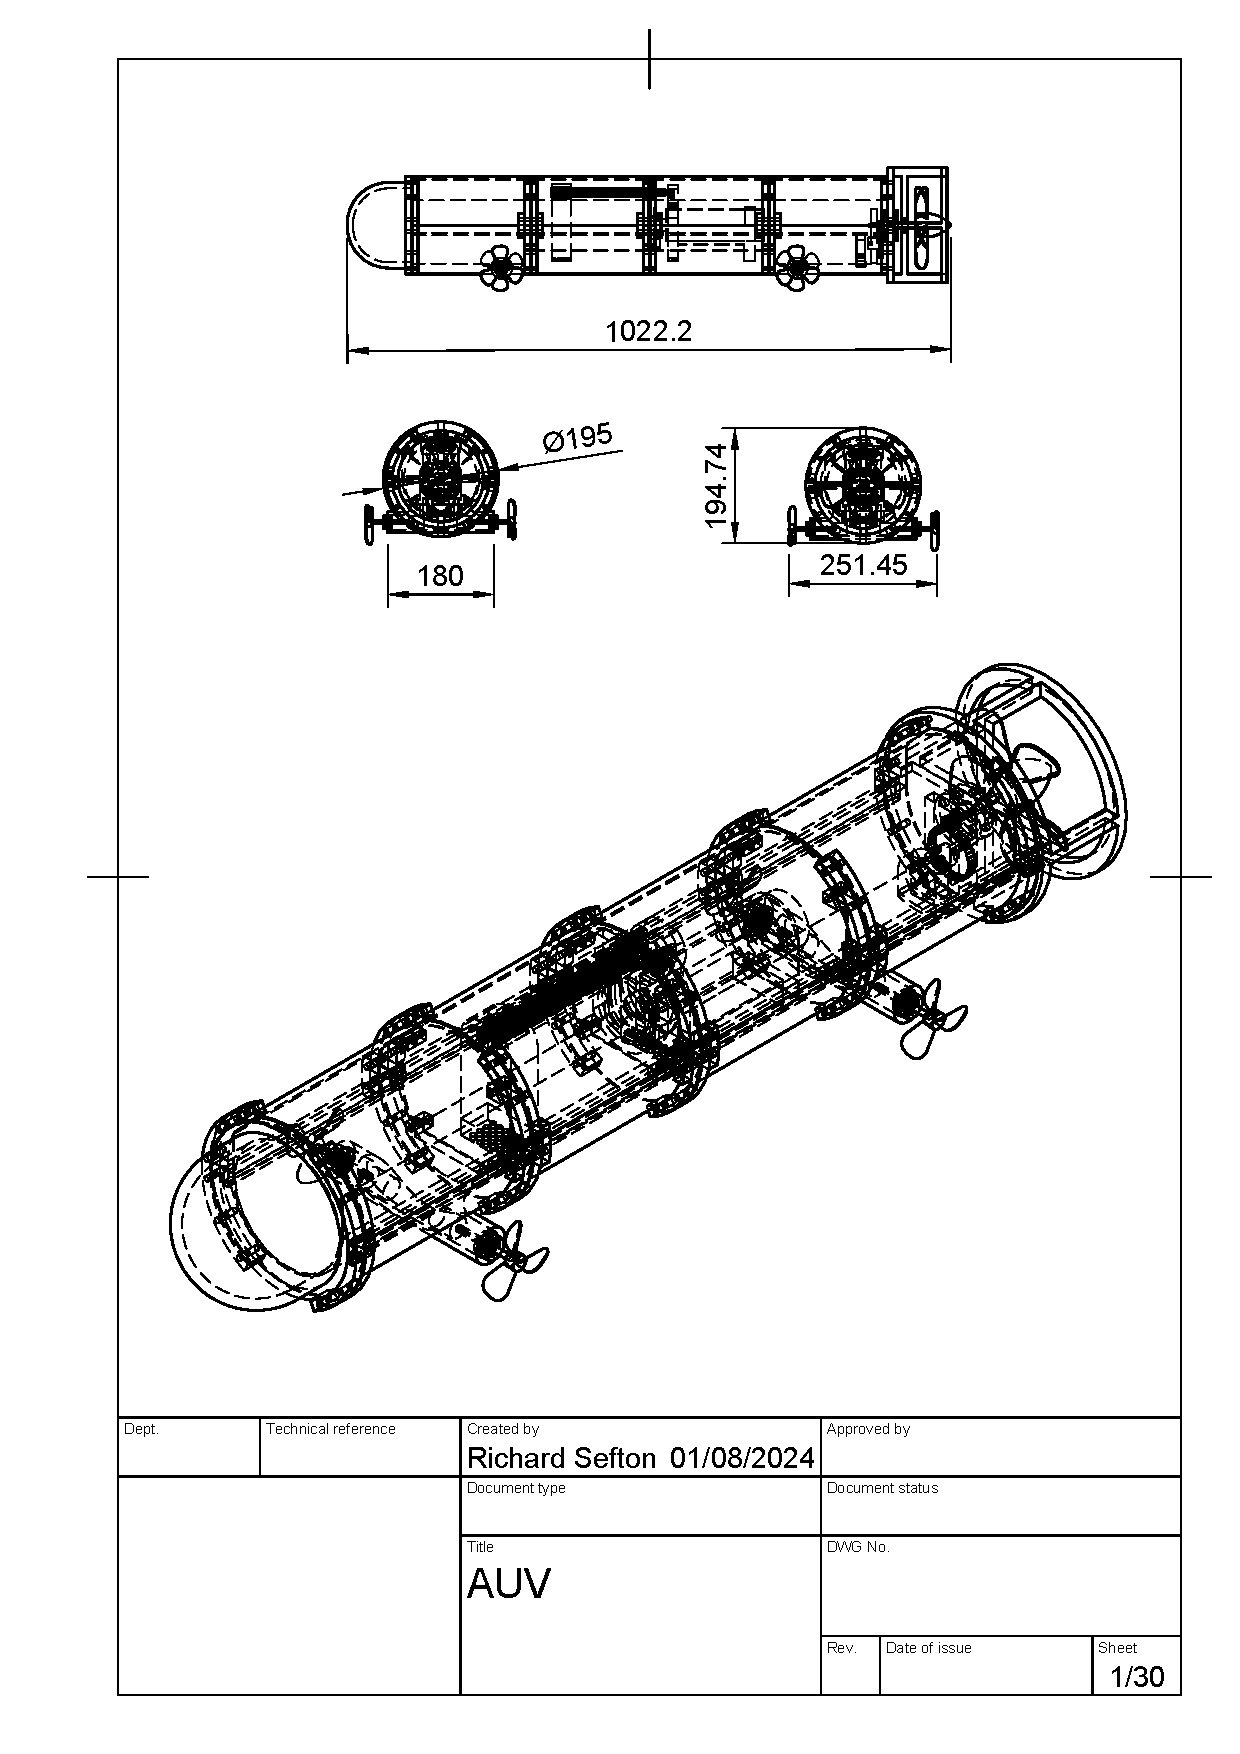
\includepdf[pages=-, width=\linewidth]{assets/AUV Drawing_Main v4.pdf}
	\end{center}
	
	\section{Final Code}\label{appendix:auv_final_code}
	
	\subsection{Common ShortTypes.h}\label{appendix:final_code_short_types_h}
	\begin{lstlisting}
		#ifndef SHORTTYPES_H
		#define	SHORTTYPES_H
		
		#include<stdint.h>
		#include <stdbool.h>
		
		typedef uint8_t u8;
		typedef int8_t i8;
		
		typedef uint16_t u16;
		typedef int16_t i16;
		
		typedef uint32_t u32;
		typedef int32_t i32;
		
		#endif	/* SHORTTYPES_H */
	\end{lstlisting}
	
	\subsection{Common Common.h}\label{appendix:final_code_common_h}
	\begin{lstlisting}
		#ifndef COMMON_H
		#define	COMMON_H
		
		#include <avr/io.h>
		#include "ShortTypes.h"
		
		extern enum {
			RED = PIN6_bm,
			GREEN = PIN5_bm,
			BLUE = PIN4_bm
		} Colours;
		
		void setupRGB(void);
		void RGB(u8);
		
		
		#endif	/* COMMON_H */
	\end{lstlisting}
	
	\subsection{Common Common.c}\label{appendix:final_code_common_c}
	\begin{lstlisting}
		#include "Common.h"
		
		void setupRGB(void) {
			PORTB.DIR |= RED | GREEN | BLUE;
			PORTB.OUT |= (RED | GREEN | BLUE);
		}
		
		void RGB(u8 colour) {
			PORTB.OUT |= RED | GREEN | BLUE;
			PORTB.OUT &= ~colour;
		}
	\end{lstlisting}
	
	\subsection{Central Controller AddressBook.h}\label{appendix:final_code_address_book_h}
	\begin{lstlisting}
		#ifndef ADDRESSBOOK_H
		#define	ADDRESSBOOK_H
		
		#define     DEPTH_CONTROLLER    0x40
		#define     US_BOTTOM           0x30
		#define     US_RIGHT            0x31
		#define     US_LEFT             0x32
		#define     US_FORWARD          0x33
		#define     FORWARD_MOTOR       0x45
		#define     LEFT_MOTOR          0x46
		#define     RIGHT_MOTOR         0x47
		
		#endif	/* ADDRESSBOOK_H */
	\end{lstlisting}
	
	\subsection{Central Controller AUV.h}\label{appendix:final_code_auv_h}
	\begin{lstlisting}		
		#ifndef MODULES_H
		#define	MODULES_H
		
		#include "ShortTypes.h"
		
		typedef enum {
			FMD_FORWARD = 1,
			FMD_STOP = 2,
			FMD_BACKWARD = 3
		} ForwardMotorDirection;
		
		typedef enum {
			SMD_NONE = 0,
			SMD_LEFT = 1,
			SMD_RIGHT = 2
		} SideMotorDirection;
		
		typedef enum {
			SMS_ON = 1,
			SMS_OFF = 2
		} SideMotorState;
		
		typedef enum {
			SD_NONE = 0,
			SD_LOWER = 1,
			SD_FORWARD = 2,
			SD_LEFT = 3,
			SD_RIGHT = 4
		} SonarDirection;
		
		typedef enum {
			LOWER = 0,
			FORWARD = 1,
			LEFT = 2,
			RIGHT = 3
		} SonarModule;
		
		typedef struct {
			u16 distance;
			SonarDirection direction;
		} Sonar;
		
		typedef enum {
			LAND = 1,
			WATER = 2,
		} SonarMode;
		
		typedef struct {
			Sonar sonars [4];
			ForwardMotorDirection mainMotorDirection;
			SonarDirection mainMotorHeldBy;
			SideMotorDirection sideMotorDirection;
			SonarDirection sideMotorHeldBy;
			u8 sonarIndex;
			SonarMode sonarMode;
			u8 secondsSubmerged;
			u8 submergeTimer;
			u8 secondsSurfaced;
			u8 surfaceTimer;
		} AUV;
		
		void AUV_init(AUV*);
		Sonar* AUV_loadSonar(AUV*, SonarModule);
		void AUV_incrementSonarIndex(AUV*);
		void AUV_setMotorDirection(AUV*, ForwardMotorDirection, SonarDirection);
		void AUV_setTurnDirection(AUV*, SideMotorState, SonarDirection);
		void AUV_setSonarMode(AUV*);
		void AUV_increaseSubmergeTimer(AUV*);
		u8 AUV_shouldSurface(AUV*);
		void AUV_increaseSurfaceTimer(AUV*);
		u8 AUV_shouldDive(AUV*);
		
		#endif	/* MODULES_H */
	\end{lstlisting}
	
	\subsection{Central Controller AUV.c}\label{appendix:final_code_auv_c}
	\begin{lstlisting}
		
		#include "AUV.h"
		#include <avr/io.h>
		
		void AUV_init(AUV* self) {
			Sonar s1, s2, s3, s4;
			s1.direction = SD_LOWER;
			s2.direction = SD_FORWARD;
			s3.direction = SD_LEFT;
			s4.direction = SD_RIGHT;
			self->sonars[0] = s1;
			self->sonars[1] = s2;
			self->sonars[2] = s3;
			self->sonars[3] = s4;
			self->sonarIndex = 0;
			self->mainMotorDirection = FMD_STOP;
			self->mainMotorHeldBy = SD_NONE;
			self->sideMotorDirection = SMD_NONE;
			self->sideMotorHeldBy = SD_NONE;
			self->submergeTimer = 120;
			self->surfaceTimer = 30;
			
			//Using pins for mode detection. Votage will mean we're in water mode. 
			//PA5(Pin 6) Will be the voltage (OUTPUT)
			PORTA.DIR |= PIN5_bm;
			PORTA.OUT |= PIN5_bm;
			//PA7(Pin 8) will be the detection pin. If high, we're in Water mode. 
			PORTA.DIR &= ~(PIN7_bm);
		}
		
		Sonar* AUV_loadSonar(AUV* self, SonarModule module) {
			return &self->sonars[module];
		}
		
		void AUV_incrementSonarIndex(AUV* self) {
			self->sonarIndex++;
			if (self->sonarIndex > 3) {
				self->sonarIndex = 0;
			}
		}
		
		void AUV_setMotorDirection(AUV* self, ForwardMotorDirection dir, SonarDirection hold) {
			self->mainMotorDirection = dir;
			self->mainMotorHeldBy = hold;
		}
		
		void AUV_setTurnDirection(AUV* self, SideMotorState dir, SonarDirection hold) {
			self->sideMotorDirection = dir;
			self->sideMotorHeldBy = hold;
		}
		
		void AUV_setSonarMode(AUV* self) {
			//Set to land mode. 
			self->sonarMode = LAND;
			//If theres voltage on the detection pin, we're in water mode. 
			if (PORTA.IN & PIN7_bm) {
				self->sonarMode = WATER;
			}
		}
		
		void AUV_increaseSubmergeTimer(AUV* self) {
			self->secondsSubmerged++;
		}
		
		u8 AUV_shouldSurface(AUV* self) {
			if (self->secondsSubmerged >= self->submergeTimer) {
				self->secondsSubmerged = 0;
				return 1;
			}
			return 0;
		}
		
		void AUV_increaseSurfaceTimer(AUV* self) {
			self->secondsSurfaced++;
		}
		
		u8 AUV_shouldDive(AUV* self) {
			if (self->secondsSurfaced >= self->surfaceTimer) {
				self->secondsSurfaced = 0;
				return 1;
			}
			return 0;
		}
	\end{lstlisting}
	
	\subsection{Central Controller CentralController.h}\label{appendix:final_code_central_controller_h}
	\begin{lstlisting}
		#define F_CPU 3333333UL
		
		#include <avr/io.h>
		#include <util/delay.h>
		#include <avr/interrupt.h>
		#include "CWire.h"
		#include "ShortTypes.h"
		#include "AddressBook.h"
		#include "AUV.h"
		#include "Common.h"
		
		u8 depth = 0;
		
		void setup(void);
		void mainClkCtrl(void);
		void setupRTC(void);
		u16 ping(SonarModule);
		void handleDistanceResponse(SonarDirection);
		u8 getDepth(void);
		void dive(u8);
		void raise(u8);
		void commandForwardMotor(ForwardMotorDirection);
		void commandSideMotors(SideMotorDirection);
		
		TwoWire twi0;
		AUV auv;
		
		int main() {
			setup();
			
			//Give other modules time to init
			RGB(RED);
			_delay_ms(2000);
			
			TwoWire_init(&twi0, &TWI0);
			TwoWire_Master_begin(&twi0);
			
			//Wait for depth controller to enter home position.
			while(getDepth() != 1) {
				RGB(RED);
				_delay_ms(1000);
			}
			
			_delay_ms(2000);
			
			RGB(GREEN); 
			
			//DIVE, DIVE, DIVE!
			dive(0xFF);
			
			sei();
			
			while(1) {
				
			}
			
			return 0;
		}
		
		void setup(void) {
			mainClkCtrl();
			setupRTC();
			setupRGB();
			AUV_init(&auv);
		}
		
		void mainClkCtrl(void) 
		{
			_PROTECTED_WRITE(CLKCTRL.MCLKCTRLA, CLKCTRL_CLKSEL_OSC20M_gc);
			_PROTECTED_WRITE(CLKCTRL.MCLKCTRLB, CLKCTRL_PDIV_6X_gc | CLKCTRL_PEN_bm);
			// F_CPU with this configuration will be 3.33MHz
		}
		
		void setupRTC(void) {
			RTC.CLKSEL = RTC_CLKSEL_INT1K_gc;
			while(RTC.STATUS);
			RTC.CTRLA |= RTC_PRESCALER_DIV1_gc;
			RTC.PER = 1024;
			while (RTC.STATUS);
			RTC.INTFLAGS |= RTC_OVF_bm;
			RTC.INTCTRL |= RTC_OVF_bm;
			while (RTC.STATUS);
			RTC.CTRLA |= RTC_RTCEN_bm;
			while (RTC.STATUS);
		}
		
		u16 ping(SonarModule module) {
			AUV_setSonarMode(&auv);
			//initiate sonar
			u8 addr = 0x00;
			switch(module) {
				case LOWER: {
					addr = US_BOTTOM;
					break;
				}
				case FORWARD: {
					addr = US_FORWARD;
					break;
				}
				case LEFT: {
					addr = US_LEFT;
					break;
				}
				case RIGHT: {
					addr = US_RIGHT;
					break;
				}
				default: break;
			}
			cli();
			TwoWire_beginTransmission(&twi0, addr);
			TwoWire_write(&twi0, auv.sonarMode); //The value is the mode of operation
			TwoWire_endTransmission(&twi0, 1);
			_delay_ms(250); //Wait before responding
			
			//get the results
			u16 dist = 0;
			TwoWire_requestFrom(&twi0, addr, 2, 1);
			if (TwoWire_available(&twi0) == 2) {
				u8 dataLow = TwoWire_read(&twi0);  
				u8 dataHigh = TwoWire_read(&twi0);
				dist = dataLow;
				dist |= (dataHigh << 8);
			}
			sei();
			
			//Becuase the sensor is mounted on the bottom, we can't actively test this now its
			//assembled. It was tested as working previously but now we need to override the 
			//returned value. 
			if ((addr == US_BOTTOM) && (auv.sonarMode == LAND)) {
				return 0xFFFF; //Return max. 
			}
			return dist;
		}
		
		void handleDistanceResponse(SonarDirection dir) {
			switch (dir) {
				case SD_LOWER: {
					Sonar* s = AUV_loadSonar(&auv, LOWER);
					if (s->distance > 0 && s->distance < 1400) {
						depth = getDepth();
						if (depth == 0) {
							//Handle later
						} else {
							/**
							* I think this is having the same ghandi bug from the civ games. 
							* if depth is less than 10 and we take off 10 it does to 255 - depth - 10
							* 
							* If its less than 10 we just need to raise to 0. 
							*/
							if (depth > 10) {
								depth -= 10;
								raise(depth);
							} else if(depth == 1) {
								raise(1); //not doing anything in reality. 
							} else {
								raise(0); //raise to 0 and it should 1 itself. 
							}                    
						}
						AUV_setMotorDirection(&auv, FMD_STOP, SD_LOWER);
					} else if (s->distance > 0 && s->distance > 3000) {
						//                if (depth < 245) {
							//                    depth += 10;
							//                    dive(depth);
							//                } else if (depth == 254) {
							//                    dive(254);
							//                } else {
							//                    dive(255);
							//                }
						if (auv.mainMotorHeldBy == SD_LOWER || auv.mainMotorHeldBy == SD_NONE) {
							AUV_setMotorDirection(&auv, FMD_FORWARD, SD_NONE);
						}
					}
				}
				
				case SD_FORWARD: {
					Sonar* s = AUV_loadSonar(&auv, FORWARD);
					if (s->distance > 0 && s->distance < 1400) {
						if(s->distance < 800) {
							AUV_setMotorDirection(&auv,FMD_BACKWARD, SD_FORWARD);
						} else {
							AUV_setMotorDirection(&auv, FMD_STOP, SD_FORWARD);
						}
					} else if(s->distance > 0 && s->distance > 1400) {
						if (auv.mainMotorHeldBy == SD_FORWARD || auv.mainMotorHeldBy == SD_NONE) {
							AUV_setMotorDirection(&auv, FMD_FORWARD, SD_NONE);
						}
					}
				}
				
				case SD_LEFT: {
					Sonar* s = AUV_loadSonar(&auv, LEFT);
					if (s->distance < 1400) {
						AUV_setMotorDirection(&auv,FMD_STOP, SD_LEFT);
						AUV_setTurnDirection(&auv, SMD_RIGHT, SD_LEFT);
					} else {
						if (auv.mainMotorHeldBy == SD_LEFT || auv.mainMotorHeldBy == SD_NONE) {
							AUV_setMotorDirection(&auv, FMD_FORWARD, SD_NONE);
						}
						if (auv.sideMotorHeldBy == SD_LEFT || auv.sideMotorHeldBy == SD_NONE) {
							AUV_setTurnDirection(&auv, SMD_NONE, SD_NONE);
						}
					}
				}
				
				case SD_RIGHT: {
					Sonar* s = AUV_loadSonar(&auv, LEFT);
					if (s->distance < 800) {
						AUV_setMotorDirection(&auv,FMD_STOP, SD_RIGHT);
						AUV_setTurnDirection(&auv, SMD_LEFT, SD_RIGHT);
					} else {
						if (auv.mainMotorHeldBy == SD_RIGHT || auv.mainMotorHeldBy == SD_NONE) {
							AUV_setMotorDirection(&auv, FMD_FORWARD, SD_NONE);
						}
						if (auv.sideMotorHeldBy == SD_RIGHT || auv.sideMotorHeldBy == SD_NONE) {
							AUV_setTurnDirection(&auv, SMD_NONE, SD_NONE);
						}
					}
				}
				
				default: { 
					break;
				}
			}
		}
		
		u8 getDepth(void) {
			RGB(BLUE);
			_delay_ms(100); //So we can see the xmission
			u8 data = 0;
			TwoWire_requestFrom(&twi0, DEPTH_CONTROLLER, 1, 1);
			if (TwoWire_available(&twi0)) {
				data = TwoWire_read(&twi0);  // Read the received byte
			}
			return data;
		}
		
		void dive(u8 d) {
			RGB(BLUE);
			TwoWire_beginTransmission(&twi0, DEPTH_CONTROLLER);
			TwoWire_write(&twi0, d);
			TwoWire_endTransmission(&twi0, 1);
			RGB(GREEN);
		}
		void raise(u8 d) {
			dive(d);
		}
		
		void commandForwardMotor(ForwardMotorDirection dir) {
			RGB(BLUE);
			TwoWire_beginTransmission(&twi0, FORWARD_MOTOR);
			TwoWire_write(&twi0, (u8)dir);
			TwoWire_endTransmission(&twi0, 1);
			RGB(GREEN);
		}
		
		void commandSideMotors(SideMotorDirection dir) {
			RGB(BLUE);
			if (dir == SMD_LEFT) {
				TwoWire_beginTransmission(&twi0, LEFT_MOTOR);
				TwoWire_write(&twi0, (u8)SMS_OFF);
				TwoWire_endTransmission(&twi0, 1);
				_delay_ms(100);
				TwoWire_beginTransmission(&twi0, RIGHT_MOTOR);
				TwoWire_write(&twi0, (u8)SMS_ON);
				TwoWire_endTransmission(&twi0, 1);
			} else if (dir == SMD_RIGHT) {
				TwoWire_beginTransmission(&twi0, RIGHT_MOTOR);
				TwoWire_write(&twi0, (u8)SMS_OFF);
				TwoWire_endTransmission(&twi0, 1);
				_delay_ms(100);
				TwoWire_beginTransmission(&twi0, LEFT_MOTOR);
				TwoWire_write(&twi0, (u8)SMS_ON);
				TwoWire_endTransmission(&twi0, 1);
			} else if (dir == SMD_NONE) {
				TwoWire_beginTransmission(&twi0, RIGHT_MOTOR);
				TwoWire_write(&twi0, (u8)SMS_OFF);
				TwoWire_endTransmission(&twi0, 1);
				_delay_ms(100);
				TwoWire_beginTransmission(&twi0, LEFT_MOTOR);
				TwoWire_write(&twi0, (u8)SMS_OFF);
				TwoWire_endTransmission(&twi0, 1);
			}
			RGB(GREEN);
		}
		
		ISR(RTC_CNT_vect) {
			RGB(BLUE);
			switch(auv.sonarIndex) {
				case LOWER: {
					auv.sonars[LOWER].distance = ping(LOWER);
					RGB(GREEN);
					handleDistanceResponse(SD_LOWER);
					break;
				}
				case FORWARD: {
					auv.sonars[FORWARD].distance = ping(FORWARD);
					RGB(GREEN);
					handleDistanceResponse(SD_FORWARD);
					break;
				}
				case LEFT: {
					auv.sonars[LEFT].distance = ping(LEFT);
					RGB(GREEN);
					handleDistanceResponse(SD_LEFT);
					break;
				}
				case RIGHT: {
					auv.sonars[RIGHT].distance = ping(RIGHT);
					RGB(GREEN);
					handleDistanceResponse(SD_RIGHT);
					break;
				}
				default: break;
			}
			AUV_incrementSonarIndex(&auv);
			commandForwardMotor(auv.mainMotorDirection);
			commandSideMotors(auv.sideMotorDirection);
			
			if ((depth == 0) || (depth == 1)) {
				AUV_increaseSurfaceTimer(&auv);
				if (AUV_shouldDive(&auv) == 1) {
					dive(255);
				}
			} else {
				AUV_increaseSubmergeTimer(&auv);
				if (AUV_shouldSurface(&auv)) {
					raise(0);
				}
			}
			
			
			RTC.INTFLAGS = RTC_OVF_bm;
		}
	\end{lstlisting}
	
	\subsection{Stepper Motor StepperMotor.h}\label{appendix:final_code_stepper_motor_h}
	\begin{lstlisting}
		#ifndef STEPPERMOTOR_H
		#define	STEPPERMOTOR_H
		
		#ifndef F_CPU
		#define F_CPU 3333333UL
		#endif
		
		#include <avr/io.h>
		#include <util/delay.h>
		#include "Common.h"
		
		/*
		* Lets apply the pins to some defines
		* 
		* 
		* 
		* StepperMotor
		* 17 - PC0
		* 18 - PC1
		* 19 - PC2
		* 20 - PC3
		* 
		* Going to use 6(PA5), 7(PA6). These need to be inputs to detect voltage
		* Will also need interrupts on these and pullup enabled because they're floating
		* 
		* Button we'll put on PB2
		* Also we'll add the pullup because while theres no voltage its also floating. 
		*/
		extern enum {
			STEP_PIN_1 = PIN0_bm,
			STEP_PIN_2 = PIN1_bm,
			STEP_PIN_3 = PIN2_bm,
			STEP_PIN_4 = PIN3_bm
		} StepperPins;
		
		typedef struct {
			i8 step;
		} StepperMotor;
		
		void StepperMotor_init(StepperMotor*);
		void StepperMotor_setup(void);
		void StepperMotor_step(StepperMotor*);
		void StepperMotor_increaseStep(StepperMotor*);
		void StepperMotor_decreaseStep(StepperMotor*);
		void StepperMotor_allStop(void);
		
		#endif	/* STEPPERMOTOR_H */
	\end{lstlisting}
	
	\subsection{Stepper Motor StepperMotor.c}\label{appendix:final_code_stepper_motor_c}
	\begin{lstlisting}
		#include "StepperMotor.h"
		
		void StepperMotor_init(StepperMotor* self) {
			StepperMotor_setup();
			self->step = 0;
		}
		
		void StepperMotor_setup(void) {
			PORTC.DIR |= STEP_PIN_1 | STEP_PIN_2 | STEP_PIN_3 | STEP_PIN_4;
		}
		
		void StepperMotor_step(StepperMotor* self) {
			switch(self->step) {
				case 0:
				PORTC.OUTCLR |= STEP_PIN_1 | STEP_PIN_2 | STEP_PIN_3;
				PORTC.OUTSET |= STEP_PIN_4;
				break;     
				case 1:
				PORTC.OUTCLR |= STEP_PIN_1 | STEP_PIN_2;
				PORTC.OUTSET |=  STEP_PIN_3 | STEP_PIN_4;
				break;    
				case 2:
				PORTC.OUTCLR |= STEP_PIN_1 | STEP_PIN_2 | STEP_PIN_4;
				PORTC.OUTSET |= STEP_PIN_3;
				break;      
				case 3:
				PORTC.OUTCLR |= STEP_PIN_1 | STEP_PIN_4;
				PORTC.OUTSET |= STEP_PIN_2 | STEP_PIN_3;
				break;  
				case 4:
				PORTC.OUTCLR |= STEP_PIN_1 | STEP_PIN_3 | STEP_PIN_4;
				PORTC.OUTSET |= STEP_PIN_2;
				break;    
				case 5:
				PORTC.OUTCLR |= STEP_PIN_3 | STEP_PIN_4;
				PORTC.OUTSET |= STEP_PIN_1 | STEP_PIN_2;
				break;
				case 6:
				PORTC.OUTCLR |= STEP_PIN_2 | STEP_PIN_3 | STEP_PIN_4;
				PORTC.OUTSET |= STEP_PIN_1;
				break;
				case 7:
				PORTC.OUTCLR |= STEP_PIN_2 | STEP_PIN_3;
				PORTC.OUTSET |= STEP_PIN_1 | STEP_PIN_4;
				break;
				default:
				break;
			}
		}
		
		void StepperMotor_increaseStep(StepperMotor* self) {
			self->step++;
			if (self->step > 7) {
				self->step = 0;
			}
		}
		
		void StepperMotor_decreaseStep(StepperMotor* self) {
			self->step--;
			if (self->step < 0) {
				self->step = 7;
			}
		}
		
		void StepperMotor_allStop(void) {
			PORTC.OUTCLR |= STEP_PIN_1 | STEP_PIN_2 | STEP_PIN_3 | STEP_PIN_4;
		}
	\end{lstlisting}
	
	\subsection{Depth Controller DepthController.h}\label{appendix:final_code_depth_controller_h}
	\begin{lstlisting}	
		#define F_CPU 3333333UL
		#include <avr/io.h>
		#include <util/delay.h>
		#include <avr/interrupt.h>
		#include "CWire.h"
		#include "ShortTypes.h"
		#include "Common.h"
		#include "StepperMotor.h"
		
		u8 plungerPos = 255;
		u8 commandedPos = 0;
		
		#define THREAD_OUT 0x01
		#define THREAD_IN 0x02
		#define STOP 0x00
		#define GO 0x01
		
		u8 dir = THREAD_IN;
		u8 run = GO;
		
		//PortA
		#define BUFFER_OUT_PIN PIN5_bm
		#define BUFFER_IN_PIN PIN7_bm
		
		//Functions we need to define. 
		//This isn't in pseudocode. I like to include it to be explicit
		void mainClkCtrl(void);
		void setup(void);
		void setupPins(void);
		void setupRTC(void);
		
		//My TWI Library requires callbacks. 
		void I2C_RX_Callback(u8);
		void I2C_TX_Callback(void);
		//Also need an address we can bind this module to. 
		
		TwoWire twi0;
		StepperMotor stepper;
		
		#define ADDR 0x40
		
		int main(void) {
			setup();
			
			TwoWire_init(&twi0, &TWI0);
			TwoWire_Slave_begin(&twi0, ADDR, 0, 0);
			
			TwoWire_onReceive(&twi0, I2C_RX_Callback);
			TwoWire_onRequest(&twi0, I2C_TX_Callback);
			
			sei();
			
			while(1) {
				if (plungerPos != commandedPos) {
					run = GO;
					RGB(BLUE);
					if ((dir == THREAD_OUT && plungerPos != 254) && plungerPos != commandedPos){
						StepperMotor_step(&stepper);
						StepperMotor_decreaseStep(&stepper);
					} else if ((dir == THREAD_IN && plungerPos != 1) && plungerPos != commandedPos) {
						StepperMotor_step(&stepper);
						StepperMotor_increaseStep(&stepper);
					}
					_delay_us(750);
				} else {
					run = STOP;
					RGB(GREEN);
					StepperMotor_allStop();
				}
			}
			
			return 0;
		}
		
		void mainClkCtrl(void) 
		{
			_PROTECTED_WRITE(CLKCTRL.MCLKCTRLA, CLKCTRL_CLKSEL_OSC20M_gc | CLKCTRL_CLKOUT_bm);
			_PROTECTED_WRITE(CLKCTRL.MCLKCTRLB, CLKCTRL_PDIV_6X_gc | CLKCTRL_PEN_bm);
		}
		
		void setup(void) {
			mainClkCtrl();
			setupRTC();
			setupPins();
			StepperMotor_init(&stepper);
			setupRGB();
		}
		
		void setupRTC(void) {
			RTC.CLKSEL = RTC_CLKSEL_INT1K_gc;
			while(RTC.STATUS);
			RTC.CTRLA |= RTC_PRESCALER_DIV1_gc;
			/**
			* End to end takes 2min 25s/145s
			* 
			* Going to knock off 5s so we should be clear of the buffer. 
			* 
			* 145/255 = 0.57 and change. So one tick of the pos is worth ~0.57s 
			*/
			RTC.PER = 582; //Needed to add 12 as 1k is 1024 kHz
			while (RTC.STATUS);
			RTC.INTFLAGS |= RTC_OVF_bm;
			RTC.INTCTRL |= RTC_OVF_bm;
			while (RTC.STATUS);
			RTC.CTRLA |= RTC_RTCEN_bm;
			while (RTC.STATUS);
		}
		
		void setupPins(void) {
			//Buffers
			PORTA.DIR &= ~(BUFFER_OUT_PIN);
			PORTA.DIR &= ~(BUFFER_IN_PIN);
			
			//This pin is for the voltage to be detected. 
			PORTA.DIR |= PIN4_bm;
			PORTA.OUT |= PIN4_bm;
			
			PORTA.PIN5CTRL |= PORT_PULLUPEN_bm | PORT_ISC_RISING_gc;
			PORTA.PIN7CTRL |= PORT_PULLUPEN_bm | PORT_ISC_RISING_gc; 
		}
		
		void I2C_RX_Callback(u8 nBytes) {
			u8 data = 0;
			while (TwoWire_available(&twi0)) {
				data = TwoWire_read(&twi0);
			}
			
			if (data > plungerPos) {
				dir = THREAD_OUT;
			} else {
				dir = THREAD_IN;
			}
			
			commandedPos = data;
		}
		
		void I2C_TX_Callback(void) {
			//This is used in read requests where the controller is expecting the depth.
			
			//without getting the current depth we would risk bottoming out particularly 
			//in the first call to dive which sends to max depth. 
			TwoWire_write(&twi0, plungerPos);
		}
		
		//ISRS
		ISR(RTC_CNT_vect) {
			RTC.INTFLAGS = RTC_OVF_bm;
			if (run == GO) {
				if (dir == THREAD_OUT) {
					plungerPos += 1;
				} else if (dir == THREAD_IN) {
					plungerPos -= 1;
				}
			} 
			//Incase we naturally get there without using the buffer. We don't want to sit at 0
			//    if (plungerPos == 1) {
				//        commandedPos = 1;
				//        dir = THREAD_IN;
				//    } else if (plungerPos == 254 && commandedPos > 0) {
				//        commandedPos = 254;
				//        dir = THREAD_OUT;
				//    }
		}
		
		ISR(PORTA_PORT_vect) {
			if (PORTA.INTFLAGS & BUFFER_OUT_PIN) {
				if (!(PORTA.IN & BUFFER_OUT_PIN)) {
					RTC.CNT = 0;
					plungerPos = 255;
					commandedPos = (254);
					dir = THREAD_IN;
				}
				PORTA.INTFLAGS |= BUFFER_OUT_PIN;
			}
			
			if (PORTA.INTFLAGS & BUFFER_IN_PIN) {
				if (!(PORTA.IN & BUFFER_IN_PIN)) {
					RTC.CNT = 0;
					plungerPos = 0;
					commandedPos = 1;
					dir = THREAD_OUT; 
				}
				PORTA.INTFLAGS |= BUFFER_IN_PIN;
			}
			PORTA.INTFLAGS |= BUFFER_IN_PIN | BUFFER_OUT_PIN;
		}
	\end{lstlisting}
	
	\subsection{Sonar Sonar.h}\label{appendix:final_code_sonar_h}
	\begin{lstlisting}
		#ifndef SONAR_H
		#define	SONAR_H
		
		/**
		Because the Sonar Module is infact multiple modules lets make it a library project 
		* and call it in when needed. 
		*/
		
		#ifndef F_CPU
		#define F_CPU 3333333UL
		#endif
		
		#include <avr/io.h>
		#include <util/delay.h>
		#include "Common.h"
		
		//typedef uint8_t u8;
		//typedef uint16_t u16;
		
		extern enum {
			TRIGGER = PIN3_bm,
			ECHO = PIN2_bm
		} S_Pins;
		
		typedef enum {
			LAND = 1,
			WATER = 2,
		} Mode;
		
		typedef struct {
			u8 as_u8;
			u16 as_u16;
			float as_float;
		} Distance;
		
		typedef struct {
			Mode mode;
			u16 ticks;
			float sos_land;
			float sos_water;
			Distance distance;
		} Sonar;
		
		void Sonar_init(Sonar*, Mode);
		void Sonar_setupSonar(void);
		void Sonar_setupTCA(void);
		void Sonar_enableTCA(void);
		void Sonar_disableTCA(void);
		void Sonar_trigger(Sonar*);
		void Sonar_calculateDistance(Sonar*);
		void Sonar_convertDistances(Sonar*);
		
		#endif	/* SONAR_H */
	\end{lstlisting}
	
	\subsection{Sonar Sonar.c}\label{appendix:final_code_sonar_c}
	\begin{lstlisting}
		#include "Sonar.h"
		
		void Sonar_init(Sonar* self, Mode mode) {
			Sonar_setupSonar();
			Sonar_setupTCA();
			self->sos_land = 34300.0f;
			self->sos_water = 148000.0f;
			self->mode = mode;
		}
		
		void Sonar_setupSonar(void) {
			PORTC.DIR |= TRIGGER;
			PORTC.DIR &= ~ECHO;
			
			PORTC.PIN1CTRL |= PORT_PULLUPEN_bm;
			PORTC.PIN2CTRL |= PORT_PULLUPEN_bm;
		}
		
		void Sonar_setupTCA(void) {
			TCA0.SINGLE.CTRLA |= TCA_SINGLE_CLKSEL_DIV1_gc;
			TCA0.SINGLE.CNT = 0;
			TCA0.SINGLE.PER = 0xFFFF;
		}
		
		void Sonar_enableTCA(void) {
			TCA0.SINGLE.CNT = 0;
			TCA0.SINGLE.CTRLA |= TCA_SINGLE_ENABLE_bm;
		}
		
		void Sonar_disableTCA(void) {
			TCA0.SINGLE.CTRLA &= ~(TCA_SINGLE_ENABLE_bm);
		}
		
		void Sonar_trigger(Sonar* self) {
			PORTC.OUTSET |= TRIGGER;
			_delay_us(10);
			PORTC.OUTCLR |= TRIGGER;
			//wait for echo to go high
			while((!(PORTC.IN & ECHO)));
			Sonar_enableTCA();
			//Wait for echo to go High
			while(PORTC.IN & ECHO);
			Sonar_disableTCA();
			self->ticks = TCA0.SINGLE.CNT;
			Sonar_calculateDistance(self);
		}
		
		void Sonar_calculateDistance(Sonar* self) {
			float cpu = (float)F_CPU / 64.0f; //Think this was using a prescaler of 64?
			float time = (float)self->ticks / cpu;
			float sos = 0.0f;
			if (self->mode == LAND) {
				sos = self->sos_land;
			} else {
				sos = self->sos_water;
			}
			self->distance.as_float = time * sos / 2.0f;
			Sonar_convertDistances(self);
		}
		
		void Sonar_convertDistances(Sonar* self) {
			//Should take the whole number of the float
			float fdist = self->distance.as_float;
			u16 u16dist = (u16)fdist;
			u8 u8dist = (u8)(u16dist / 100);
			
			self->distance.as_u16 = u16dist;
			self->distance.as_u8 = u8dist;
		}
	\end{lstlisting}
	
	\subsection{Sonar SonarModule.h}\label{appendix:final_code_sonar_module_h}
	\begin{lstlisting}
		#include <stdint.h>
		#define F_CPU 3333333UL
		
		#include <avr/io.h>
		#include <util/delay.h>
		#include <avr/interrupt.h>
		#include "ShortTypes.h"
		#include "CWire.h"
		#include "Common.h"
		#include "Sonar.h"
		
		void setup(void);
		void mainClkCtrl(void);
		
		//TWI Library requires callbacks. 
		void I2C_RX_Callback(u8);
		void I2C_TX_Callback(void);
		//Also need an address 
		#define ADDR 0x30
		
		TwoWire twi0;
		Sonar sonar;
		
		int main(void) {
			setup();
			RGB(RED);
			
			TwoWire_init(&twi0, &TWI0);
			TwoWire_Slave_begin(&twi0, ADDR, 0, 0);
			
			TwoWire_onReceive(&twi0, I2C_RX_Callback);
			TwoWire_onRequest(&twi0, I2C_TX_Callback);
			
			sei();
			
			RGB(GREEN);
			
			while(1) {
				//Do nothing. 
			}
		}
		
		void setup(void) {
			mainClkCtrl();
			Sonar_init(&sonar, LAND);
			setupRGB();
		}
		
		void mainClkCtrl(void) {
			_PROTECTED_WRITE(CLKCTRL.MCLKCTRLA, CLKCTRL_CLKSEL_OSC20M_gc | CLKCTRL_CLKOUT_bm);
			_PROTECTED_WRITE(CLKCTRL.MCLKCTRLB, CLKCTRL_PDIV_6X_gc | CLKCTRL_PEN_bm);
		}
		
		void I2C_RX_Callback(u8 val) {
			/**
			* So the i2c rail isn't waiting for a response and runs a risk of timing out:
			* 
			* We are going to trigger the ping from the master with a write command. 
			* Once triggered the master will wait (a time in ms, maybe 200ms) then 
			* perform a read request to get the results. 
			*/
			if (val == 0x01) { //We're only expecting 1 byte
				while (TwoWire_available(&twi0)) {
					u8 data = TwoWire_read(&twi0);
					//arbitrary value just to prevent against accidental triggers from noise on the line
					if ((data == LAND) || (data == WATER)) { 
						if (data == LAND) {
							sonar.mode = LAND;
						} else if (data == WATER) {
							sonar.mode == WATER;
						}
						RGB(BLUE);
						Sonar_trigger(&sonar);
					}
				}
			}
		}
		
		//By the point this is called the distance calculations should have occurred.
		void I2C_TX_Callback(void) {
			//sending it back as the u16 value. Should really do this in the library but lets just check it works first. 
			u8 high = sonar.distance.as_u16 >> 8;
			u8 low = sonar.distance.as_u16;
			u8 dataToSend [2] = { low, high };
			TwoWire_writeBytes(&twi0, dataToSend, 2);
			RGB(GREEN);
		}
	\end{lstlisting}
	
	\subsection{Main Motor MainMotor.h}\label{appendix:final_code_main_motor_h}
	\begin{lstlisting}
		#define F_CPU 3333333UL
		
		#include <avr/io.h>
		#include <util/delay.h>
		#include <avr/interrupt.h>
		#include "Common.h"
		#include "StepperMotor.h"
		#include "CWire.h"
		#include "ShortTypes.h"
		
		#define ADDR 0x45
		
		void setup(void);
		//TWI Library requires callbacks. 
		void I2C_RX_Callback(u8);
		
		typedef enum {
			FORWARD = 1,
			STOP = 2,
			BACKWARD = 3
		} Directions;
		
		StepperMotor stepper;
		Directions dir;
		TwoWire twi0;
		
		int main() {
			setup();
			
			RGB(RED);
			
			TwoWire_init(&twi0, &TWI0);
			TwoWire_Slave_begin(&twi0, ADDR, 0, 0);
			
			TwoWire_onReceive(&twi0, I2C_RX_Callback);
			
			RGB(GREEN);
			dir = STOP;
			
			sei();
			
			while(1) {
				if (dir == FORWARD) {
					RGB(GREEN);
					StepperMotor_step(&stepper);
					StepperMotor_increaseStep(&stepper);
				} else if (dir == BACKWARD) {
					RGB(BLUE);
					StepperMotor_step(&stepper);
					StepperMotor_decreaseStep(&stepper);
				} else {
					RGB(RED);
					StepperMotor_allStop();
				}
				_delay_us(750);
			}
			
			return 0;
		}
		
		void setup(void) {
			setupRGB();
			StepperMotor_init(&stepper);
		}
		
		//TWI Library requires callbacks. 
		void I2C_RX_Callback(u8 numOfBytes) {
			if (numOfBytes == 1) {
				while (TwoWire_available(&twi0)) {
					u8 data = TwoWire_read(&twi0);
					if (data == FORWARD) {
						dir = FORWARD;
					} 
					if (data == BACKWARD) {
						dir = BACKWARD;
					}
					if (data == STOP) {
						dir = STOP;
					}
				}
			}
		}
	\end{lstlisting}
	
	\subsection{Side Motor SideMotor.h}\label{appendix:final_code_side_motor_h}
	\begin{lstlisting}
		#define F_CPU 3333333UL
		
		#include <avr/io.h>
		#include <avr/interrupt.h>
		#include "CWire.h"
		#include "Common.h"
		#include "ShortTypes.h"
		#include <util/delay.h>
		
		#define ADDR 0x46
		
		void setup(void);
		void setupPins(void);
		void startMotors(void);
		void stopMotors(void);
		void I2C_RX_Callback(u8);
		
		#define MOTOR1_PIN1 PIN0_bm
		#define MOTOR1_PIN2 PIN1_bm
		#define MOTOR2_PIN1 PIN2_bm
		#define MOTOR2_PIN2 PIN3_bm
		
		enum MotorState {
			ON = 1,
			OFF = 2
		};
		
		TwoWire twi0;
		int main(void) {
			setup();
			
			TwoWire_init(&twi0, &TWI0);
			TwoWire_Slave_begin(&twi0, ADDR, 0, 0);
			
			TwoWire_onReceive(&twi0, I2C_RX_Callback);
			
			sei();
			
			RGB(RED);
			
			while(1) {
				
			}
			
			return 0;
		}
		
		void setup(void) {
			setupRGB();
			setupPins();
		}
		
		void setupPins(void) {
			PORTC.DIR |= MOTOR1_PIN1 | MOTOR1_PIN2 | MOTOR2_PIN1 | MOTOR2_PIN2;
			PORTC.OUTCLR = MOTOR1_PIN1 | MOTOR1_PIN2 | MOTOR2_PIN1 | MOTOR2_PIN2;
		}
		
		void startMotors(void) {
			PORTC.OUTSET = MOTOR1_PIN1 | MOTOR2_PIN1;
			PORTC.OUTCLR = MOTOR1_PIN2 | MOTOR2_PIN2;
		}
		
		void stopMotors(void) {
			PORTC.OUTCLR = MOTOR1_PIN1 | MOTOR1_PIN2 | MOTOR2_PIN1 | MOTOR2_PIN2;
		}
		
		void I2C_RX_Callback(u8 numBytes) {
			if (numBytes == 1) {
				while (TwoWire_available(&twi0)) {
					u8 data = TwoWire_read(&twi0);
					if (data == ON) {
						RGB(GREEN);
						startMotors();
					} else if (data == OFF) {
						RGB(RED);
						stopMotors();
					}
				}
			}
		}
	\end{lstlisting}
\end{document}